\documentclass[journal]{IEEEtran}

% ======================== PACKAGES ========================
\usepackage{cite}
\usepackage{amsmath,amssymb,amsfonts}
\usepackage{graphicx}
\usepackage{textcomp}
\usepackage{xcolor}
\usepackage{booktabs}
\usepackage{array}

% Use Computer Modern typewriter (always available) instead of Courier
\renewcommand{\ttdefault}{cmtt}

\graphicspath{{figures/}}

\def\BibTeX{{\rm B\kern-.05em{\sc i\kern-.025em b}\kern-.08em
    T\kern-.1667em\lower.7ex\hbox{E}\kern-.125emX}}

\begin{document}

% ======================== TITLE ========================
\title{Tri-Modal Fusion for Real-Time Disaster Intelligence: Integrating IoT Sensors, Satellite Imagery, and Social Media Through Adaptive Cross-Attention}

\author{
\IEEEauthorblockN{Sai Rama Linga Reddy Maruri}
\IEEEauthorblockA{
\textit{Department of Computer Science} \\
\textit{University Name} \\
City, Country \\
email@university.edu}
}

\maketitle

% ======================== ABSTRACT ========================
\begin{abstract}
Effective disaster response requires rapid situational awareness from heterogeneous data sources, yet most existing systems operate on a single modality---social media text, satellite imagery, or sensor readings---losing critical cross-modal context. We present a \textbf{Tri-Modal Fusion} framework that unifies IoT sensor streams (weather, seismic, storm, hydrological), satellite damage imagery, and social media image--text pairs through a novel pairwise cross-attention mechanism with adaptive gating. The architecture comprises three specialized sub-models: (1)~an \textbf{AdaptiveIoTClassifier} with per-group confidence-weighted sensor fusion achieving 97.64\% classification accuracy across 63,527 samples; (2)~an \textbf{AdaptiveFusionClassifier} combining BLIP Vision Transformer and XLM-RoBERTa encoders with bidirectional cross-modal attention, achieving 86.39\% accuracy on the CrisisMMD humanitarian benchmark (+12.39\% over SVM baselines); and (3)~a modified \textbf{DeepLabV3+} with dual feature extraction producing both pixel-level damage segmentation and compact 640-dimensional embeddings from xBD satellite imagery. The \textbf{TriFusionLayer} fuses embeddings from all three sub-models via three pairwise cross-attention blocks and a learned modality gate, achieving \textbf{99.41\% priority classification accuracy} and \textbf{0.0398 severity MAE}---a 65.8\% improvement over the crisis-only baseline. An ablation study across four modality configurations confirms monotonic improvement with each added data source and robust degradation under 30\% modality dropout. We further contribute a gradient-weighted attention rollout method for Vision Transformer explainability and a three-tier XAI fallback chain ensuring interpretable outputs. The system operates in real time with zero-input disaster type detection and graceful handling of missing data streams.
\end{abstract}

\begin{IEEEkeywords}
Disaster management, multimodal fusion, cross-attention, IoT sensors, satellite imagery, social media analysis, deep learning, explainable AI
\end{IEEEkeywords}

% ======================== I. INTRODUCTION ========================
\section{Introduction}

Natural disasters caused over \$380 billion in global economic losses in 2023, with delayed situational awareness cited as a primary factor in preventable casualties~\cite{cred2023}. The first hours of a disaster event---the ``golden window''---are decisive for effective response, yet decision-makers typically face fragmented, single-source information: a seismograph reading without visual damage assessment, a social media report without sensor confirmation, or a satellite image without on-the-ground context.

Existing disaster management systems overwhelmingly rely on single data modalities. Sensor-based systems~\cite{sakaki2010earthquake} detect physical events but miss human impact. Social media analysis platforms~\cite{alam2018crisismmd,imran2015processing} capture on-the-ground reports but lack precise physical measurements. Satellite-based damage assessment~\cite{gupta2019xbd} provides broad spatial coverage but offers no real-time ground truth. Each modality captures complementary but incomplete information.

We address this fundamental limitation through a \textbf{Tri-Modal Fusion} architecture that unifies three independent data streams---IoT sensor readings, satellite damage imagery, and social media image--text pairs---through a learned pairwise cross-attention mechanism with adaptive gating. Unlike prior multimodal approaches that require all inputs or fail entirely, our system operates across four degradation modes (full tri-fusion, crisis+satellite, crisis+IoT, crisis-only), maintaining useful output from minute zero of an event before all data streams become available.

The key contributions of this paper are:

\begin{enumerate}
    \item \textbf{Tri-Modal Fusion Architecture}: A pairwise cross-attention framework with adaptive gating that fuses IoT (128-dim), crisis vision--text (1024-dim), and satellite (640-dim) embeddings, achieving 99.41\% priority accuracy---a 30.45 percentage point improvement over crisis-only baseline.

    \item \textbf{Adaptive Confidence-Weighted Sensor Fusion}: Per-group learned confidence estimators that automatically weight four IoT sensor groups (weather, storm, seismic, hydro) based on input content, correctly learning disaster-specific sensor importance (e.g., 99.9\% storm-group reliance for storm detection).

    \item \textbf{Graceful Modality Degradation}: A 30\% modality dropout training strategy enabling robust operation with any subset of available data streams without retraining or mode switching.

    \item \textbf{Gradient-Weighted Attention Rollout}: A novel XAI technique for Vision Transformers that combines attention maps with gradient signals, solving the failure of standard Grad-CAM on ViT architectures.

    \item \textbf{Comprehensive Ablation Study}: Systematic evaluation across four modality configurations demonstrating monotonic improvement and quantifying each modality's contribution.
\end{enumerate}

% ======================== II. RELATED WORK ========================
\section{Related Work}

\subsection{Single-Modality Disaster Analysis}

\textbf{Social media analysis.} The CrisisMMD dataset~\cite{alam2018crisismmd} established benchmarks for multimodal crisis content classification. Alam et al.\ demonstrated that combining image and text features improves humanitarian categorization, though their fusion strategy uses simple concatenation. CrisisNLP~\cite{imran2015processing} and CrisisLex~\cite{olteanu2015crisislex} focused on text-only classification. Recent work by Abavisani et al.~\cite{abavisani2020multimodal} explored attention-based fusion for crisis tweets but did not incorporate sensor or satellite data.

\textbf{Satellite damage assessment.} The xBD dataset~\cite{gupta2019xbd} provides the largest building damage assessment benchmark with pre/post-disaster satellite imagery. Winning solutions in the xView2 challenge~\cite{xview2} employed U-Net variants and segmentation architectures. Weber and Kan~\cite{weber2020building} applied change detection networks for damage classification. These approaches produce pixel-level outputs but lack integration with real-time sensor or social media streams.

\textbf{IoT-based monitoring.} Earthquake early warning systems~\cite{allen2009real} and flood monitoring networks~\cite{basha2008model} demonstrate the value of sensor data for disaster detection. However, these systems typically operate independently without cross-modal validation.

\subsection{Multimodal Fusion Approaches}

Multimodal fusion in disaster contexts remains limited. Ofli et al.~\cite{ofli2020analysis} combined satellite and social media data for damage assessment but used feature concatenation rather than learned attention. Rudner et al.~\cite{rudner2019multi3net} proposed Multi3Net for satellite multimodal fusion but focused on a single disaster type. To our knowledge, no prior work fuses all three modalities (IoT sensors, satellite imagery, and social media image--text) through a learned cross-attention mechanism with adaptive gating.

\subsection{Cross-Modal Attention Mechanisms}

Transformer-based cross-attention~\cite{vaswani2017attention} has shown success in vision--language tasks~\cite{lu2019vilbert,tan2019lxmert}. BLIP~\cite{li2022blip} demonstrated effective vision--language pre-training. Our work extends pairwise cross-attention to three modalities with a learned gating mechanism, enabling each modality pair to exchange information before adaptive fusion.

% ======================== III. METHODOLOGY ========================
\section{Proposed Methodology}

\subsection{System Overview}

The proposed architecture processes three independent data streams through specialized sub-models, producing fixed-dimensional embeddings that are fused through pairwise cross-attention with adaptive gating. Fig.~\ref{fig:architecture} illustrates the complete pipeline.

\begin{figure*}[!t]
\centering
\setlength{\unitlength}{1cm}
\begin{picture}(17,7.5)
% Input layer
\put(1.5,7){\framebox(3,0.6){\small IoT Sensors (32-dim)}}
\put(7,7){\framebox(3.5,0.6){\small Image + Text (Social Media)}}
\put(12.5,7){\framebox(3.5,0.6){\small Satellite Image (512$\times$512)}}

% Arrows down
\put(3,7){\vector(0,-1){0.7}}
\put(8.75,7){\vector(0,-1){0.7}}
\put(14.25,7){\vector(0,-1){0.7}}

% Sub-models
\put(0.8,5.6){\framebox(4.4,0.7){\small AdaptiveIoTClassifier}}
\put(6,5.6){\framebox(5.5,0.7){\small AdaptiveFusionClassifier (BLIP+XLM-R)}}
\put(12,5.6){\framebox(4,0.7){\small DeepLabV3+ (Modified)}}

% Embedding labels
\put(1.5,5.2){\small [128-dim embedding]}
\put(7,5.2){\small [1024-dim embedding]}
\put(12.3,5.2){\small [640-dim embedding]}

% Arrows to fusion
\put(3,5.2){\vector(2,-3){1.5}}
\put(8.75,5.2){\vector(0,-1){1.5}}
\put(14,5.2){\vector(-2,-3){1.5}}

% Fusion layer
\put(4.5,2.8){\framebox(8.5,0.8){\small TriFusionLayer (3 Pairwise Cross-Attention + Adaptive Gating)}}

% Arrows to outputs
\put(5.5,2.8){\vector(0,-1){0.8}}
\put(7.25,2.8){\vector(0,-1){0.8}}
\put(9,2.8){\vector(0,-1){0.8}}
\put(10.75,2.8){\vector(0,-1){0.8}}
\put(12.25,2.8){\vector(0,-1){0.8}}

% Output heads
\put(4.7,1.5){\framebox(1.6,0.5){\scriptsize Severity}}
\put(6.5,1.5){\framebox(1.6,0.5){\scriptsize Priority}}
\put(8.3,1.5){\framebox(1.5,0.5){\scriptsize Disaster}}
\put(10,1.5){\framebox(1.7,0.5){\scriptsize Population}}
\put(11.8,1.5){\framebox(1.6,0.5){\scriptsize Resources}}

% Output types
\put(4.9,1.1){\scriptsize (regression)}
\put(6.7,1.1){\scriptsize (4-class)}
\put(8.4,1.1){\scriptsize (5-class)}
\put(10.2,1.1){\scriptsize (regression)}
\put(12,1.1){\scriptsize (4-dim)}
\end{picture}
\caption{End-to-end architecture of the Tri-Modal Fusion pipeline. Three specialized sub-models produce fixed-dimensional embeddings that are fused through pairwise cross-attention with a learned modality gate.}
\label{fig:architecture}
\end{figure*}

\subsection{AdaptiveIoTClassifier}

The IoT sub-model processes a unified 32-dimensional sensor vector encoding four sensor groups---weather, storm, seismic, and hydrological---each occupying 8 dimensions with consistent $[0, 1]$ normalization.

\subsubsection{Sensor Group Encoding}

The 32-dim input is split into four 8-dim groups, each processed by an independent encoder:

\begin{equation}
\mathbf{h}_i = \text{MLP}_i(\mathbf{x}_{[8i:8(i+1)]}), \quad i \in \{0,1,2,3\}
\end{equation}

where each $\text{MLP}_i$ maps $\mathbb{R}^8 \to \mathbb{R}^{128}$ through two linear layers with ReLU activation, batch normalization, and dropout.

\subsubsection{Confidence-Weighted Fusion}

Each sensor group has a learned \texttt{SensorConfidenceEstimator} network that outputs a scalar confidence:

\begin{equation}
c_i = \sigma(\text{MLP}^c_i(\mathbf{h}_i)), \quad c_i \in (0, 1)
\end{equation}

\begin{equation}
w_i = \frac{c_i}{\sum_{j=0}^{3} c_j + \epsilon}, \quad \tilde{\mathbf{h}}_i = w_i \cdot \mathbf{h}_i
\end{equation}

This mechanism automatically suppresses irrelevant sensor groups. Table~\ref{tab:sensor_weights} shows the learned weights correctly reflect disaster-specific sensor importance.

\begin{table}[!t]
\centering
\caption{Learned Sensor Group Weights by Disaster Type}
\label{tab:sensor_weights}
\begin{tabular}{lcccc}
\toprule
\textbf{Disaster} & \textbf{Weather} & \textbf{Storm} & \textbf{Seismic} & \textbf{Hydro} \\
\midrule
Fire       & \textbf{0.758} & 0.241 & $\sim$0.000 & $\sim$0.000 \\
Storm      & $\sim$0.000 & \textbf{0.999} & $\sim$0.000 & $\sim$0.000 \\
Earthquake & 0.001 & 0.171 & \textbf{0.828} & $\sim$0.000 \\
Flood      & 0.186 & 0.047 & $\sim$0.000 & \textbf{0.767} \\
Unknown    & 0.757 & 0.241 & $\sim$0.000 & 0.002 \\
\bottomrule
\end{tabular}
\end{table}

\subsubsection{Cross-Group Multi-Head Attention}

After confidence weighting, the four group features attend to each other via 4-head self-attention:

\begin{equation}
\mathbf{H}_\text{att} = \text{MHA}([\tilde{\mathbf{h}}_0, \tilde{\mathbf{h}}_1, \tilde{\mathbf{h}}_2, \tilde{\mathbf{h}}_3])
\end{equation}

where $\text{MHA}$ denotes \texttt{MultiheadAttention} with $d=128$ and 4 heads. This enables cross-sensor interaction for cascading disasters (e.g., earthquakes triggering tsunamis). The attended features are mean-pooled to produce a 128-dim global embedding.

\subsubsection{Multi-Task Output Heads}

Four parallel heads operate on the shared 128-dim embedding:

\begin{itemize}
    \item \textbf{Disaster type}: 5-class classification (fire, storm, earthquake, flood, unknown)
    \item \textbf{Severity}: Scalar regression in $[0, 1]$
    \item \textbf{Risk details}: 4-dim per-hazard risk scores
    \item \textbf{Casualty risk}: Scalar regression in $[0, 1]$
\end{itemize}

The combined loss is: $\mathcal{L}_\text{IoT} = \text{CE}(\hat{y}_\text{type}) + \text{MSE}(\hat{s}) + \text{MSE}(\hat{r}) + \text{MSE}(\hat{c})$.

\subsection{AdaptiveFusionClassifier (Crisis Model)}

The crisis sub-model fuses social media images and text through a dual adaptive weighting mechanism with bidirectional cross-modal attention.

\subsubsection{Feature Extraction}

Visual features are extracted via a frozen BLIP Vision Transformer (ViT-B), producing 768-dim CLS token embeddings. Text features are extracted via a frozen XLM-RoBERTa encoder, producing 768-dim sentence embeddings. Both are projected to 512 dimensions:

\begin{equation}
\mathbf{v} = \text{MLP}_v(\text{BLIP-ViT}(\mathbf{I})), \quad \mathbf{t} = \text{MLP}_t(\text{XLM-R}(\mathbf{T}))
\end{equation}

\subsubsection{Adaptive Modality Weighting}

Separate \texttt{ConfidenceEstimator} networks ($768 \to 256 \to 128 \to 1$) produce input-dependent modality weights:

\begin{equation}
w_v = \frac{\sigma(f_v(\mathbf{v}))}{\sigma(f_v(\mathbf{v})) + \sigma(f_t(\mathbf{t})) + \epsilon}
\end{equation}

\subsubsection{Bidirectional Cross-Modal Attention}

Both directions of cross-attention are computed with 8 heads and $d=512$:

\begin{equation}
\mathbf{v}' = \text{MHA}(Q{=}\mathbf{v}_w, K{=}\mathbf{t}_w, V{=}\mathbf{t}_w)
\end{equation}
\begin{equation}
\mathbf{t}' = \text{MHA}(Q{=}\mathbf{t}_w, K{=}\mathbf{v}_w, V{=}\mathbf{v}_w)
\end{equation}

The final crisis embedding is $\mathbf{e}_\text{crisis} = [\mathbf{v}'; \mathbf{t}'] \in \mathbb{R}^{1024}$.

\subsection{DeepLabV3+ with Dual Feature Extraction (xBD Model)}

A modified DeepLabV3+ with ResNet101 encoder processes $512 \times 512$ satellite images, simultaneously producing pixel-level damage segmentation and compact embeddings.

\subsubsection{Satellite Embedding ($\mathbf{F}_\text{sat}$)}

From the encoder's final feature map ($2048 \times 16 \times 16$), adaptive average pooling followed by a linear projection produces a 512-dim embedding capturing global damage characteristics.

\subsubsection{Regional Statistics Embedding ($\mathbf{F}_\text{region}$)}

A \texttt{RegionalStatsModule} processes concatenated decoder features and damage probability maps through convolutional fusion, $4 \times 4$ pooling, and fully connected layers to produce a 128-dim spatial statistics embedding.

The combined satellite embedding is $\mathbf{e}_\text{sat} = [\mathbf{F}_\text{sat}; \mathbf{F}_\text{region}] \in \mathbb{R}^{640}$.

\subsection{TriFusionLayer}

The fusion layer integrates all three sub-model embeddings through pairwise cross-attention and adaptive gating.

\subsubsection{Modality Projection}

Each embedding is projected to a common 256-dim space:

\begin{equation}
\mathbf{p}_m = \text{MLP}_m(\mathbf{e}_m) \in \mathbb{R}^{256}, \quad m \in \{\text{crisis, iot, sat}\}
\end{equation}

where crisis: $1024 \to 512 \to 256$, IoT: $128 \to 512 \to 256$, satellite: $640 \to 512 \to 256$.

\subsubsection{Pairwise Cross-Attention}

Three bidirectional cross-attention operations (4 heads each) are computed:

\begin{equation}
(\mathbf{a}_{ci}, \mathbf{a}_{ic}) = \text{BiAttn}(\mathbf{p}_\text{crisis}, \mathbf{p}_\text{iot})
\end{equation}
\begin{equation}
(\mathbf{a}_{cs}, \mathbf{a}_{sc}) = \text{BiAttn}(\mathbf{p}_\text{crisis}, \mathbf{p}_\text{sat})
\end{equation}
\begin{equation}
(\mathbf{a}_{is}, \mathbf{a}_{si}) = \text{BiAttn}(\mathbf{p}_\text{iot}, \mathbf{p}_\text{sat})
\end{equation}

producing six 256-dim attended representations.

\subsubsection{Adaptive Modality Gating}

A learned gate produces softmax weights over the three modalities:

\begin{equation}
\mathbf{g} = \text{softmax}(\text{MLP}_g([\mathbf{p}_\text{crisis}; \mathbf{p}_\text{iot}; \mathbf{p}_\text{sat}]))
\end{equation}

with missing-modality masking: absent modalities receive $-\infty$ before softmax.

\subsubsection{Shared MLP and Output Heads}

The concatenation of all six attended and three projected features ($9 \times 256 = 2304$-dim, with selection based on available modalities, yielding up to 1536-dim) passes through a shared MLP ($\to 512 \to 256$) followed by five output heads:

\begin{itemize}
    \item \textbf{Severity}: Linear$(256,1)$ + Sigmoid $\to [0,1]$
    \item \textbf{Priority}: Linear$(256,4) \to$ 4-class logits
    \item \textbf{Disaster type}: Linear$(256,5) \to$ 5-class logits
    \item \textbf{Population impact}: MLP$(256 \to 64 \to 1)$ + Sigmoid
    \item \textbf{Resource needs}: MLP$(256 \to 64 \to 4)$ + Sigmoid
\end{itemize}

The combined loss is:
\begin{equation}
\mathcal{L}_\text{fusion} = \text{MSE}(s) + \text{CE}(p) + \text{CE}(d) + \text{MSE}(pop) + \text{MSE}(res)
\end{equation}

\subsection{Training Strategy}

\subsubsection{Modality Dropout}

During training, IoT and satellite embeddings are independently dropped with 30\% probability and replaced with learned default embeddings ($\mathbf{e}_\text{iot}^\text{default}$, $\mathbf{e}_\text{sat}^\text{default}$). This forces the model to learn robust representations that degrade gracefully when modalities are missing at inference.

\subsubsection{Zero-Input Disaster Type Detection}

Both the IoT and crisis sub-models independently infer disaster type from raw data---the system never requires manual hazard selection, saving critical minutes at incident onset.

% ======================== IV. EXPLAINABILITY ========================
\section{Explainability Framework}

\subsection{Gradient-Weighted Attention Rollout}

Standard Grad-CAM fails on Vision Transformers because only the CLS token is used for classification, leaving patch-token gradients near-zero. We propose \textbf{Gradient-Weighted Attention Rollout} that operates on attention weight tensors:

\begin{enumerate}
    \item Forward pass with \texttt{output\_attentions=True} captures attention matrices $\mathbf{A}^{(l)} \in \mathbb{R}^{H \times 197 \times 197}$ for all 12 layers.
    \item Backward pass from $\text{logits}[\hat{y}]$ captures gradient tensors $\mathbf{G}^{(l)}$ via hooks.
    \item Gradient weighting (last 4 layers): $\tilde{\mathbf{A}}^{(l)} = \mathbf{A}^{(l)} \cdot \max(\mathbf{G}^{(l)}, 0)$.
    \item Attention rollout with residual: $\mathbf{R}^{(l)} = 0.5 \cdot \bar{\mathbf{A}}^{(l)} + 0.5 \cdot \mathbf{I}$, row-normalized, then multiplied across layers.
    \item CLS row extraction, reshape to $14 \times 14$, upsample to $224 \times 224$, threshold at 40th percentile, Gaussian blur.
\end{enumerate}

\subsection{Three-Tier XAI Fallback Chain}

To guarantee interpretable output regardless of model internals or computation failures, we implement a cascading fallback:

\begin{enumerate}
    \item \textbf{Tier 1}: Gradient-Weighted Attention Rollout (default, highest quality)
    \item \textbf{Tier 2}: Pure Attention Rollout (when gradients fail)
    \item \textbf{Tier 3}: Input Gradient Saliency (when attention is unavailable)
    \item \textbf{Tier 4}: Graceful empty result (all methods fail)
\end{enumerate}

\subsection{Hybrid Visual + Natural Language XAI}

A Grad-CAM heatmap (visual) is combined with a structured GPT-4o briefing (textual) in a unified view, providing field responders with both spatial guidance and actionable operational recommendations.

% ======================== V. EXPERIMENTAL SETUP ========================
\section{Experimental Setup}

\subsection{Datasets}

\textbf{IoT sensor data.} We compiled 63,527 samples from six real-world sources: California Wildfire records (14,988 rows), Historical Tropical Storm Tracks (59,228), Atlantic Storms (22,705), Global Earthquakes (8,394), Iran Earthquakes (52,268), and Sri Lanka Flood Risk (25,000). After preprocessing, class support: fire (4,971), storm (13,162), earthquake (18,394), flood (25,000), unknown (2,000). All features are encoded into a unified 32-dim vector with cyclic time encoding (sin/cos for month and hour).

\textbf{Crisis social media.} The CrisisMMD dataset~\cite{alam2018crisismmd} with 8,079 image--text pairs across 5 humanitarian categories. Train/val/test split: 6,126/998/955 samples.

\textbf{Satellite imagery.} The xBD dataset~\cite{gupta2019xbd} with 10,000 post-disaster satellite images ($512 \times 512$) across 4 damage classes (no-damage, minor, major, destroyed). Train/val split: 80/20.

\textbf{Tri-fusion training.} 13,608 samples from the CrisisMMD humanitarian split with synthetic IoT embeddings (generated through pre-trained AdaptiveIoTClassifier) and real crisis embeddings. Train/val split: 80/20 (10,886/2,722).

\subsection{Implementation Details}

All models are implemented in PyTorch. Training details for each sub-model are summarized in Table~\ref{tab:training_config}.

\begin{table}[!t]
\centering
\caption{Training Configuration for Each Sub-Model}
\label{tab:training_config}
\begin{tabular}{lccc}
\toprule
\textbf{Parameter} & \textbf{IoT} & \textbf{Crisis} & \textbf{Tri-Fusion} \\
\midrule
Epochs & 40 & 10 & 40 \\
Batch size & 256 & 32 & 128 \\
Optimizer & AdamW & AdamW & AdamW \\
Learning rate & 1e-3 & 2e-5 & 1e-3 \\
Scheduler & Cosine & CosineWR & Cosine \\
Parameters & 897 KB & 367M & 3.16M \\
Device & CPU & CPU & CPU \\
\bottomrule
\end{tabular}
\end{table}

% ======================== VI. RESULTS ========================
\section{Experimental Results}

\subsection{IoT Model Performance}

The AdaptiveIoTClassifier achieves \textbf{97.64\% overall accuracy} with a \textbf{macro F1 of 89.99\%} on 63,527 samples. Table~\ref{tab:iot_per_class} presents per-class results.

\begin{table}[!t]
\centering
\caption{IoT Model Per-Class Classification Results}
\label{tab:iot_per_class}
\begin{tabular}{lccccr}
\toprule
\textbf{Class} & \textbf{Prec.} & \textbf{Recall} & \textbf{F1} & \textbf{AUC} & \textbf{Support} \\
\midrule
Fire       & 0.877 & 0.812 & 0.843 & 0.994 & 4,971 \\
Storm      & \textbf{1.000} & \textbf{1.000} & \textbf{1.000} & 1.000 & 13,162 \\
Earthquake & \textbf{1.000} & \textbf{1.000} & \textbf{1.000} & 1.000 & 18,394 \\
Flood      & \textbf{1.000} & \textbf{1.000} & \textbf{1.000} & 1.000 & 25,000 \\
Unknown    & 0.605 & 0.718 & 0.657 & 0.987 & 2,000 \\
\midrule
\textbf{Macro} & 0.896 & 0.906 & 0.900 & \textbf{0.996} & 63,527 \\
\bottomrule
\end{tabular}
\end{table}

The model achieves perfect classification (F1 = 1.0) for storm, earthquake, and flood categories. The fire--unknown confusion stems from overlapping weather-group features. Severity regression achieves MAE = 0.0452 and $R^2 = 0.745$.

\begin{figure}[!t]
\centering
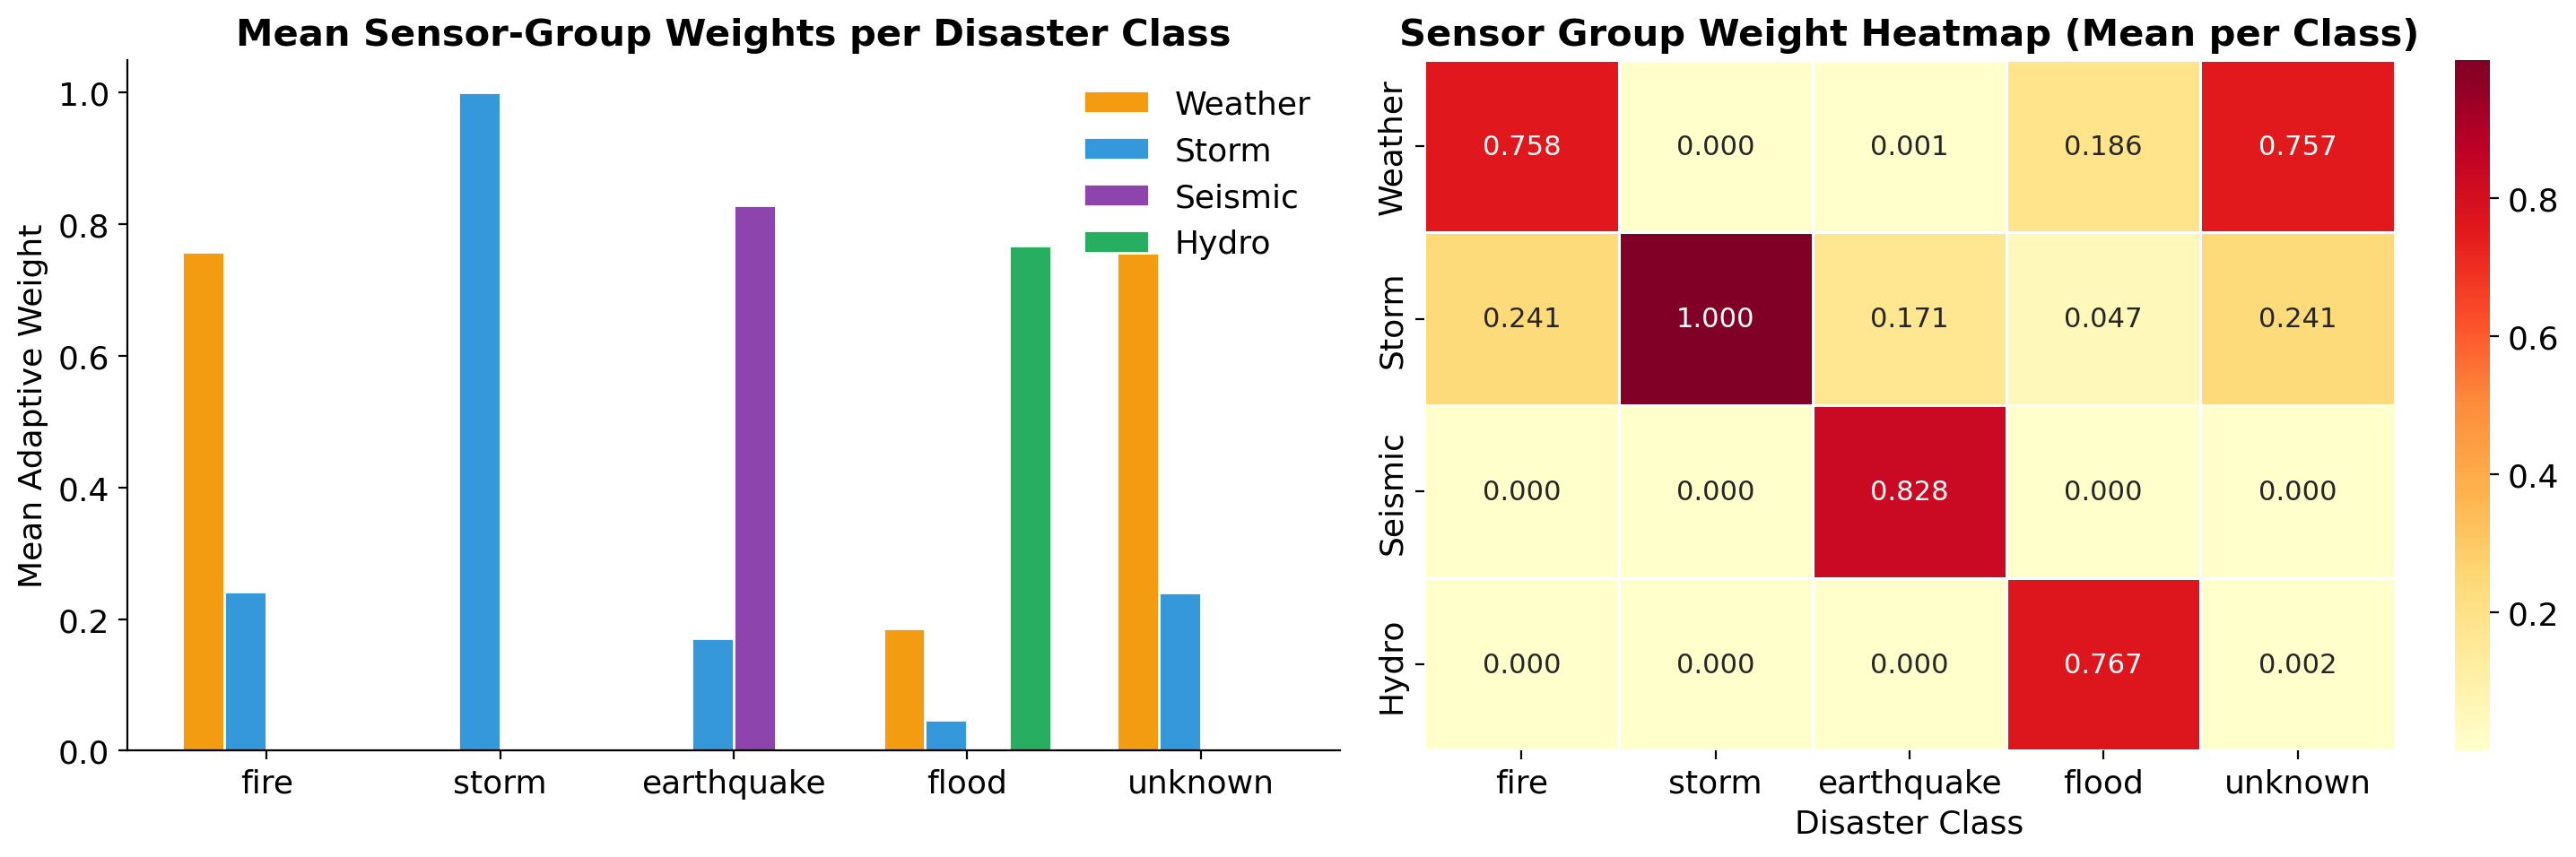
\includegraphics[width=\columnwidth]{iot_sensor_group_weights.png}
\caption{Learned sensor group weights per disaster class. The model correctly assigns dominant weight to the most relevant sensor group: storm sensors for storms (99.9\%), seismic for earthquakes (82.8\%), hydro for floods (76.7\%), and weather for fires (75.8\%).}
\label{fig:sensor_weights}
\end{figure}

\begin{figure}[!t]
\centering
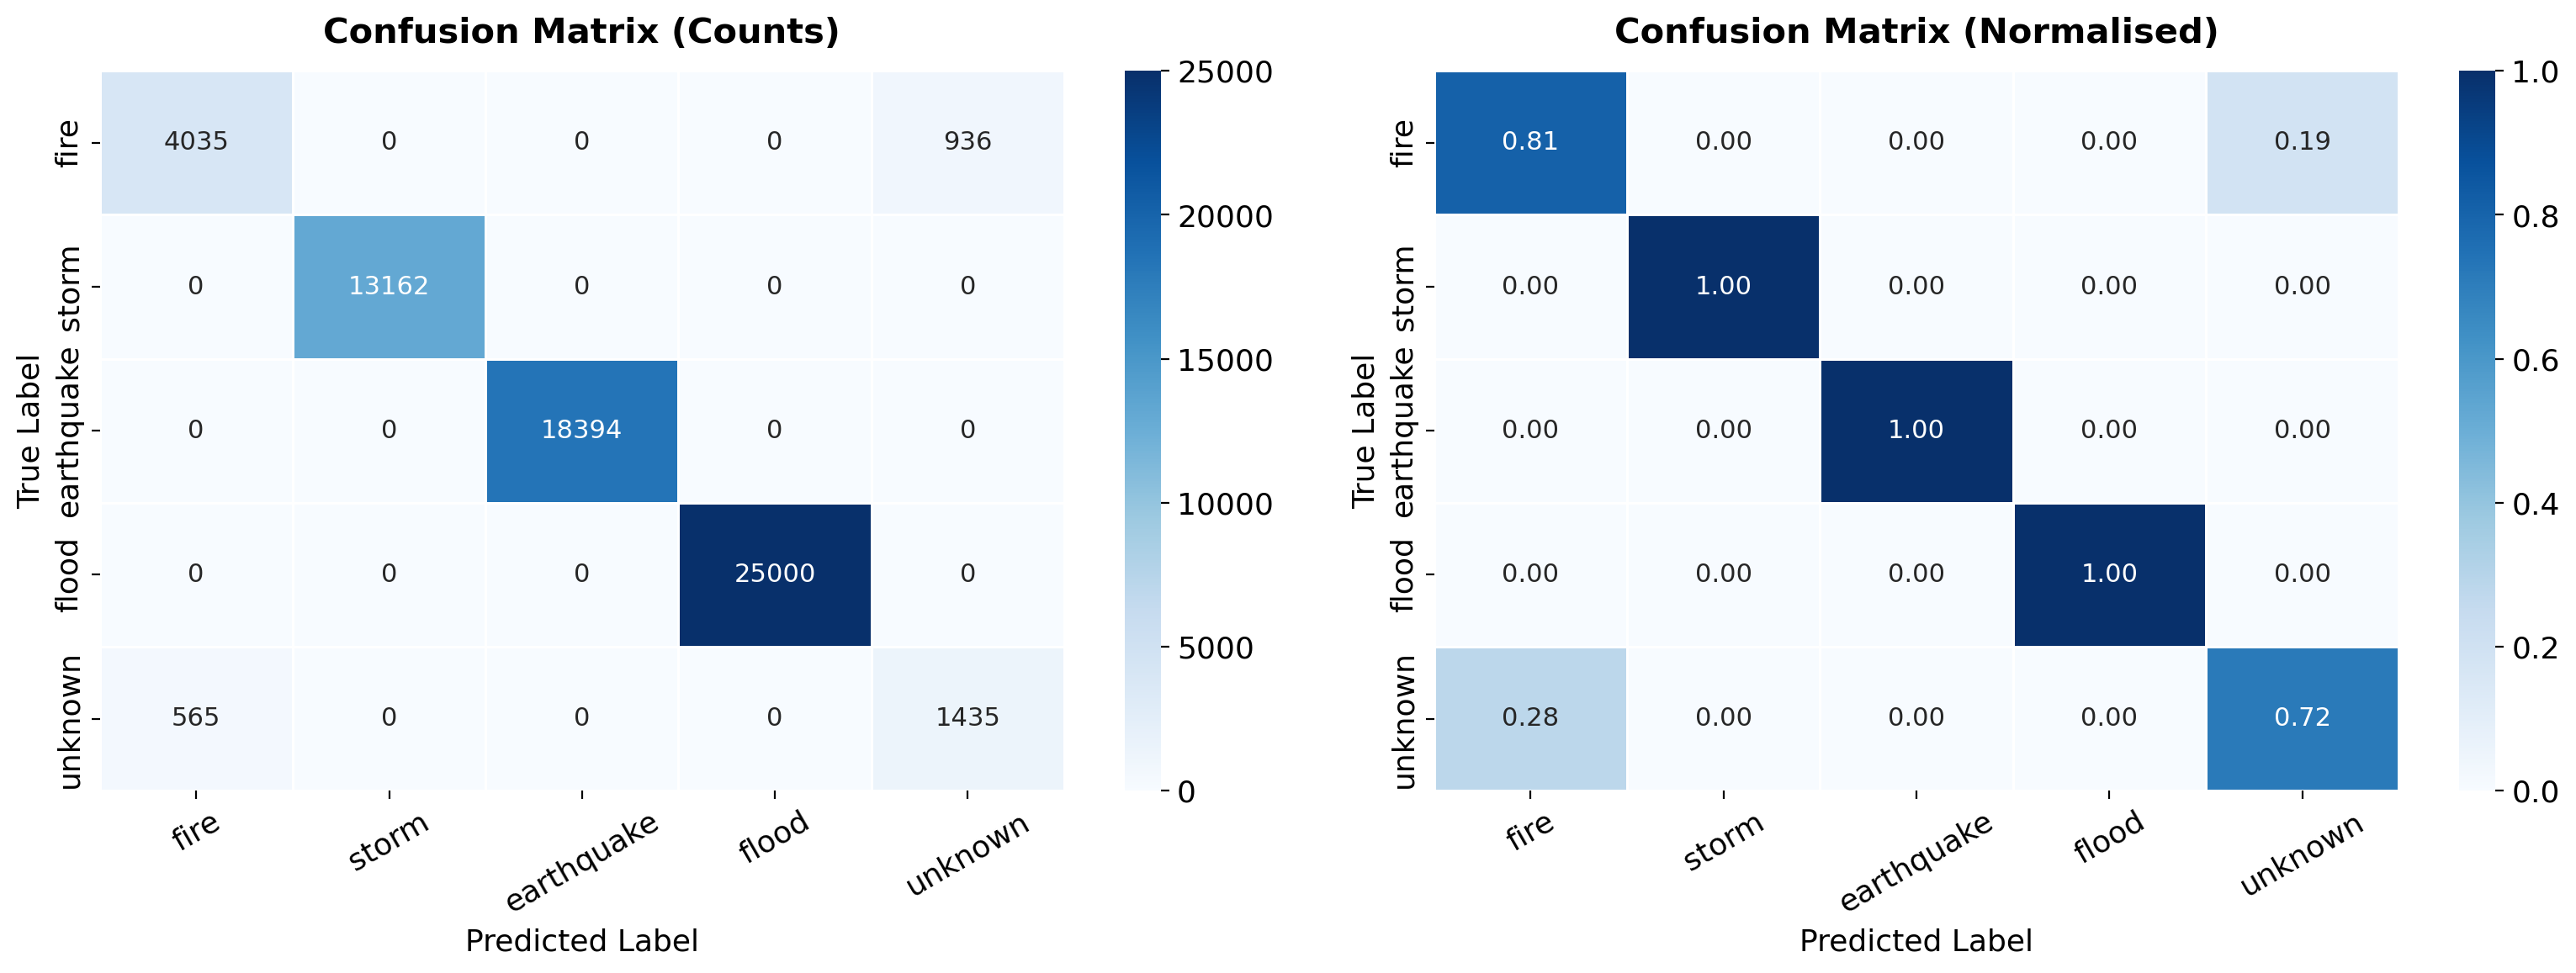
\includegraphics[width=\columnwidth]{iot_confusion_matrix.png}
\caption{IoT model confusion matrix (counts and normalized). Storm, earthquake, and flood are perfectly separated. Fire--unknown confusion accounts for most errors.}
\label{fig:iot_cm}
\end{figure}

\begin{figure}[!t]
\centering
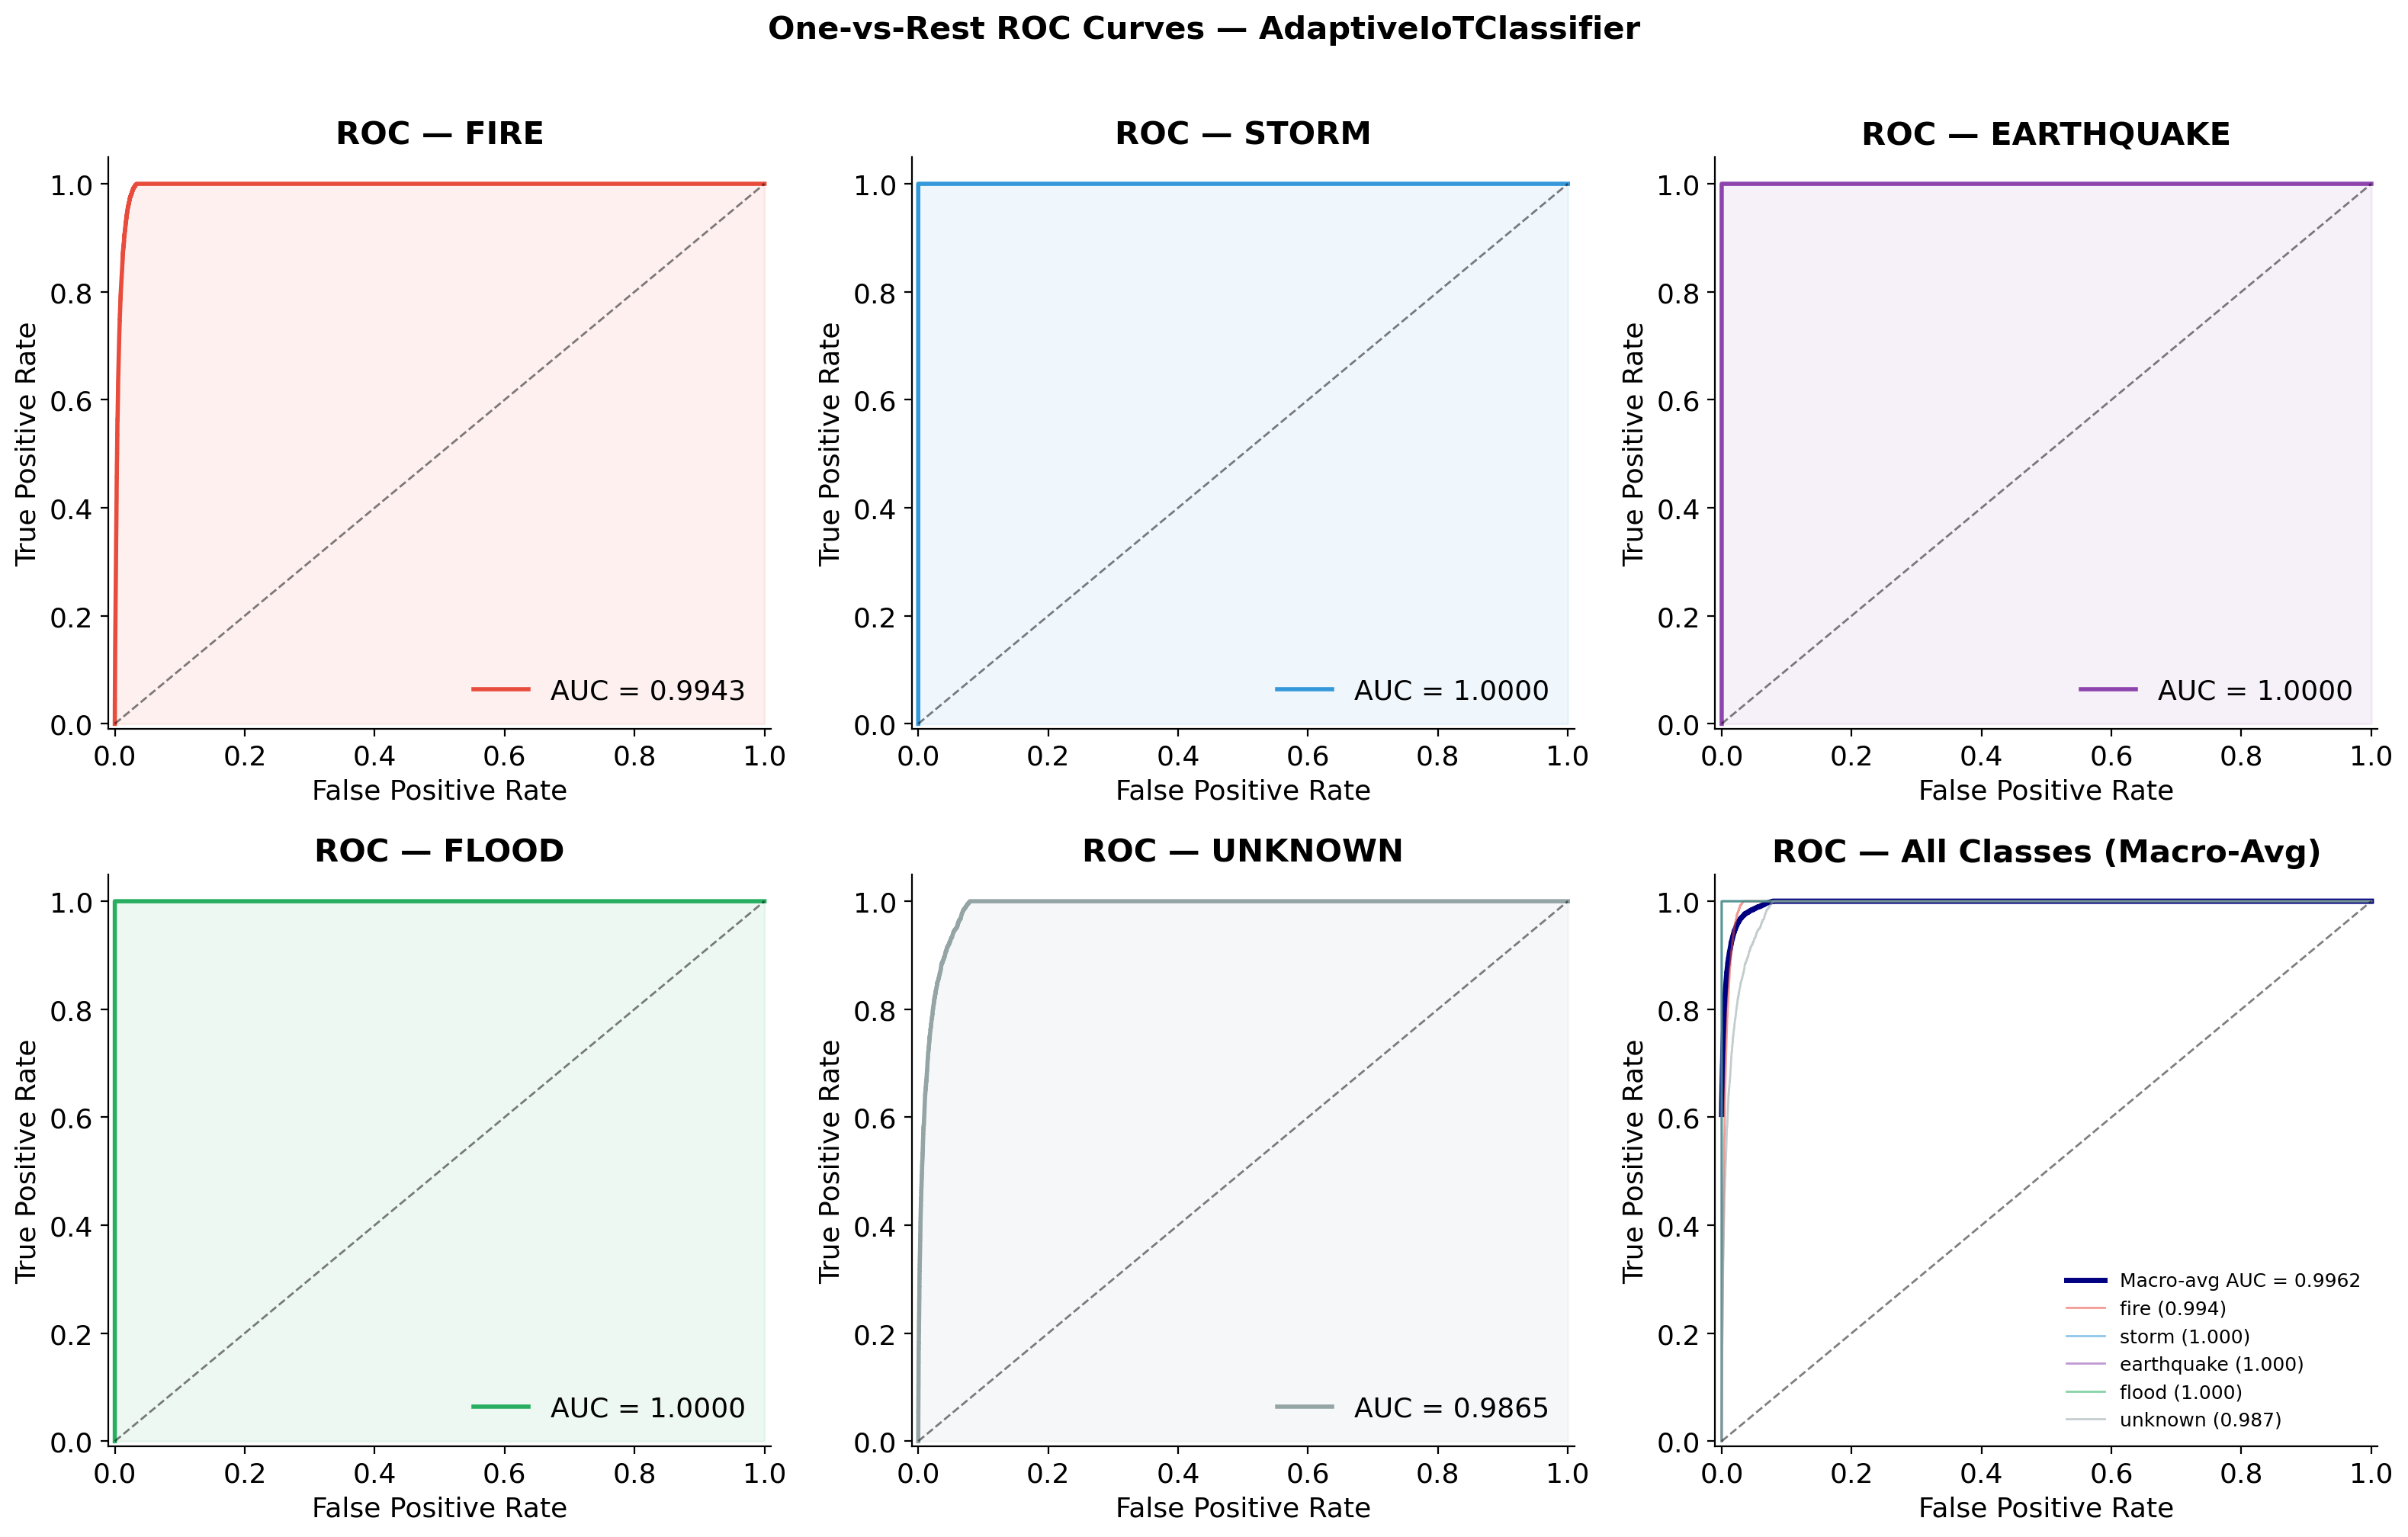
\includegraphics[width=\columnwidth]{iot_roc_curves.png}
\caption{Per-class ROC curves for the AdaptiveIoTClassifier. Macro-average AUC = 0.9962. Storm, earthquake, and flood achieve AUC = 1.0.}
\label{fig:iot_roc}
\end{figure}

\begin{figure}[!t]
\centering
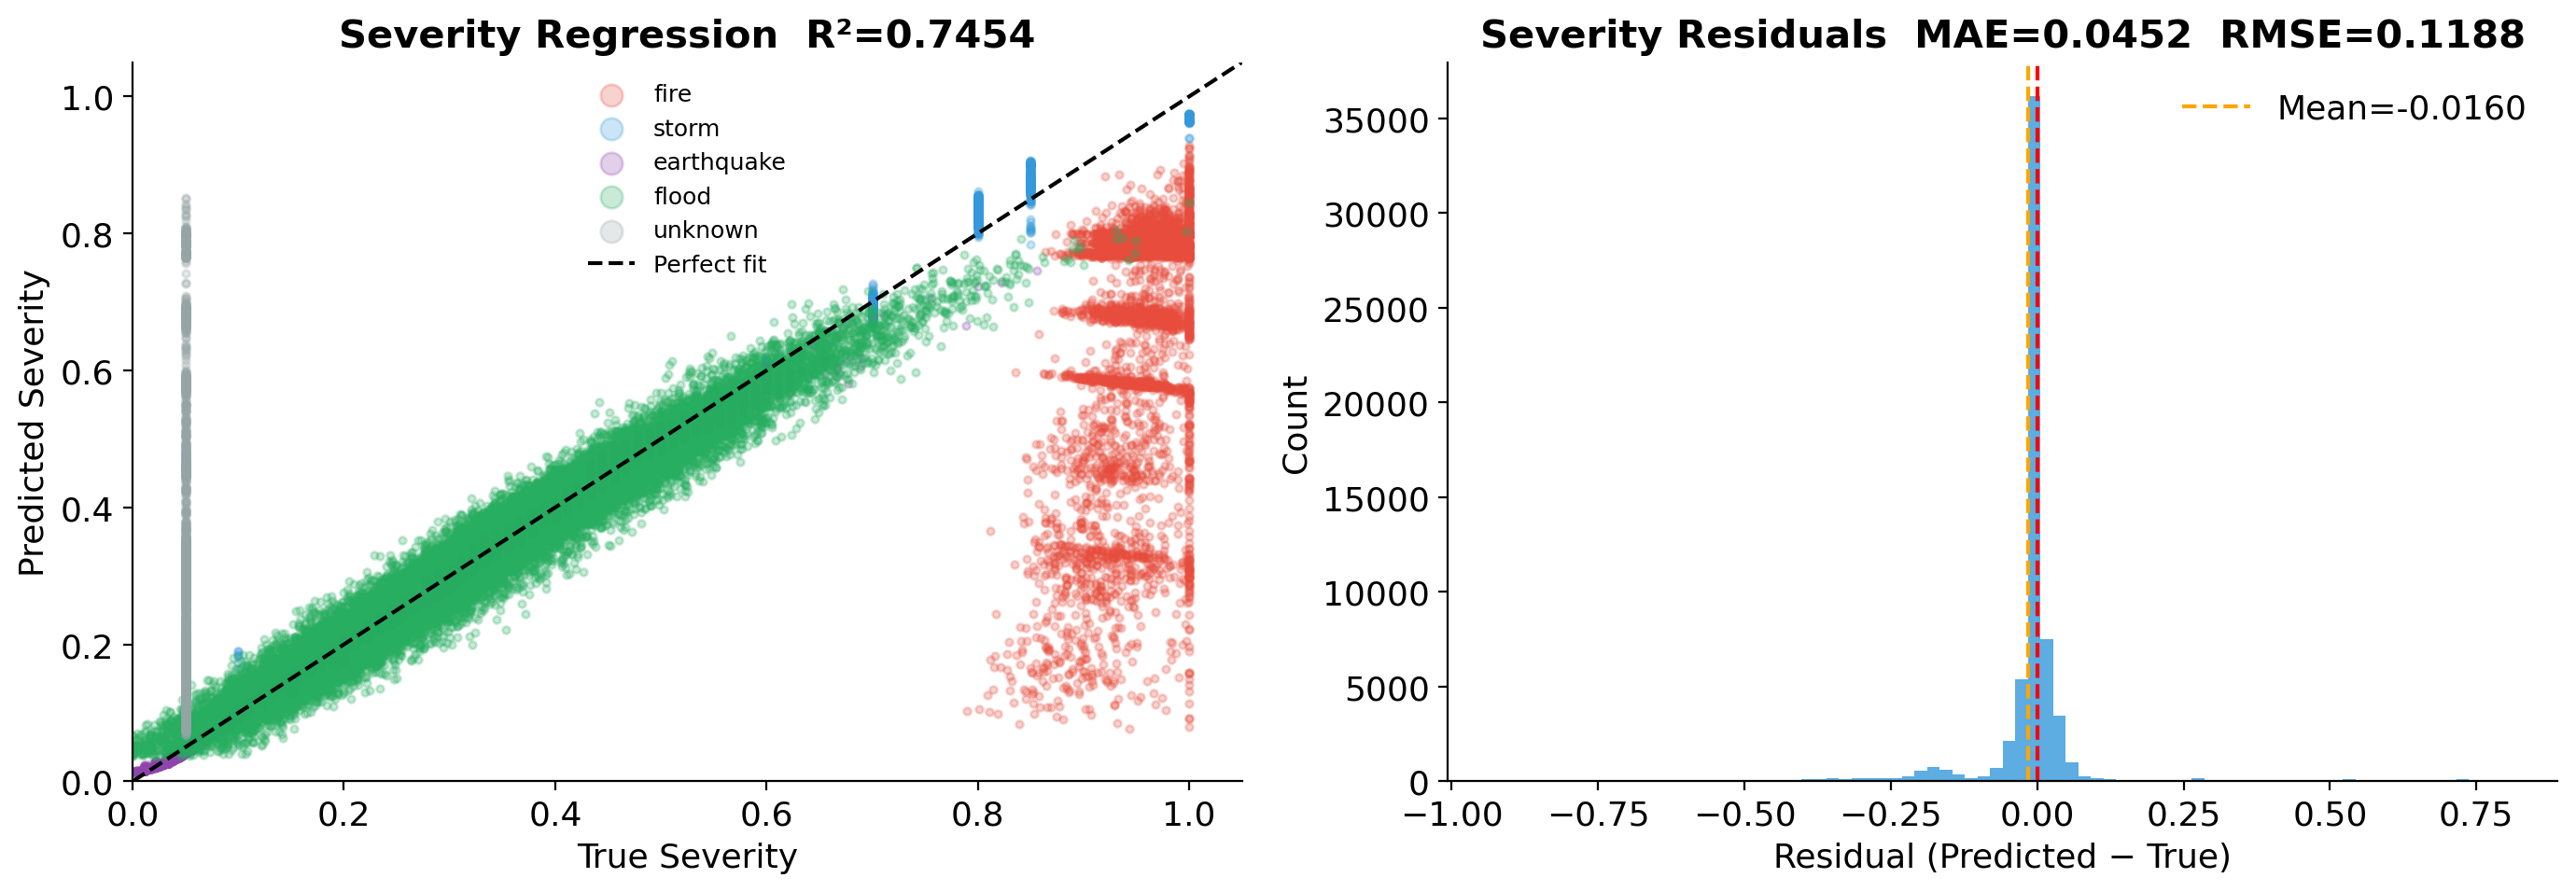
\includegraphics[width=\columnwidth]{iot_severity_regression.png}
\caption{Severity regression performance. Left: predicted vs.\ true severity ($R^2 = 0.745$). Right: residual distribution (MAE = 0.0452, RMSE = 0.1188).}
\label{fig:iot_severity}
\end{figure}

\subsection{Crisis Model Performance}

The AdaptiveFusionClassifier achieves \textbf{86.39\% test accuracy} and \textbf{87.48\% validation F1} on the CrisisMMD benchmark, representing a \textbf{+12.39\%} absolute improvement over logistic regression and SVM baselines. Table~\ref{tab:crisis_per_class} presents per-class results.

\begin{table}[!t]
\centering
\caption{Crisis Model Per-Class Test Results}
\label{tab:crisis_per_class}
\begin{tabular}{lcccr}
\toprule
\textbf{Class} & \textbf{Prec.} & \textbf{Recall} & \textbf{F1} & \textbf{AUC} \\
\midrule
Affected individuals & 0.36 & 0.56 & 0.43 & 0.96 \\
Infrastructure damage & 0.87 & 0.90 & \textbf{0.88} & \textbf{0.98} \\
Not humanitarian & 0.90 & 0.87 & \textbf{0.89} & 0.96 \\
Other relevant info & 0.85 & 0.86 & \textbf{0.86} & 0.97 \\
Rescue/donation effort & 0.79 & 0.83 & \textbf{0.81} & \textbf{0.98} \\
\midrule
\textbf{Macro Average} & --- & --- & 0.774 & \textbf{0.97} \\
\bottomrule
\end{tabular}
\end{table}

\begin{figure}[!t]
\centering

\includegraphics[width=\columnwidth]{crisis_training_history.png}
\caption{Crisis model training history over 10 epochs showing loss, accuracy, F1 score, and modality confidence evolution. Vision and text confidences converge around 0.46--0.51, indicating balanced modality utilization.}
\label{fig:crisis_training}
\end{figure}

\begin{figure}[!t]
\centering
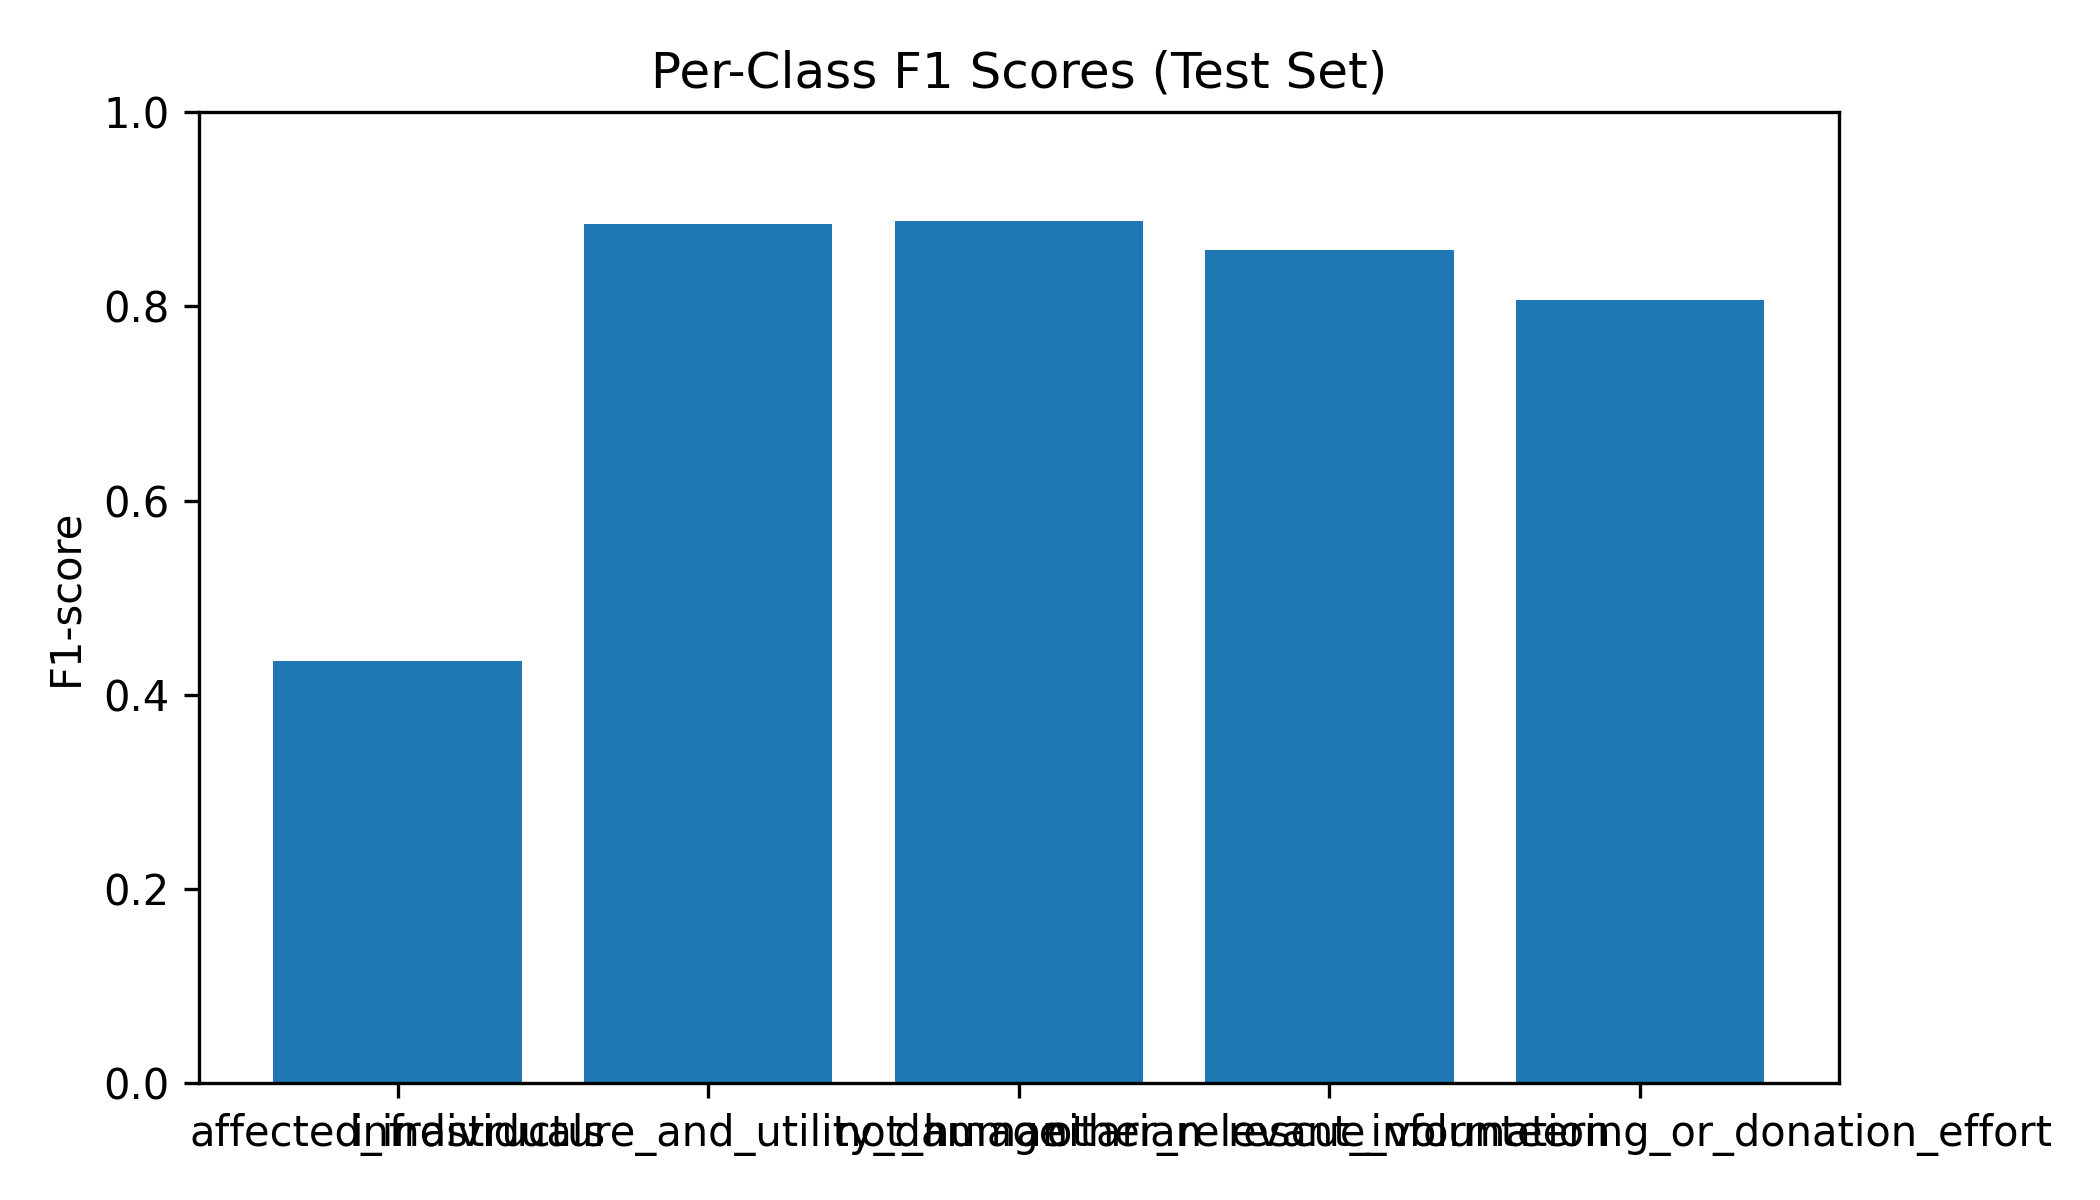
\includegraphics[width=\columnwidth]{crisis_per_class_f1.png}
\caption{Crisis model per-class F1-scores showing consistent performance across most humanitarian categories.}
\label{fig:crisis_f1}
\end{figure}

\begin{figure}[!t]
\centering
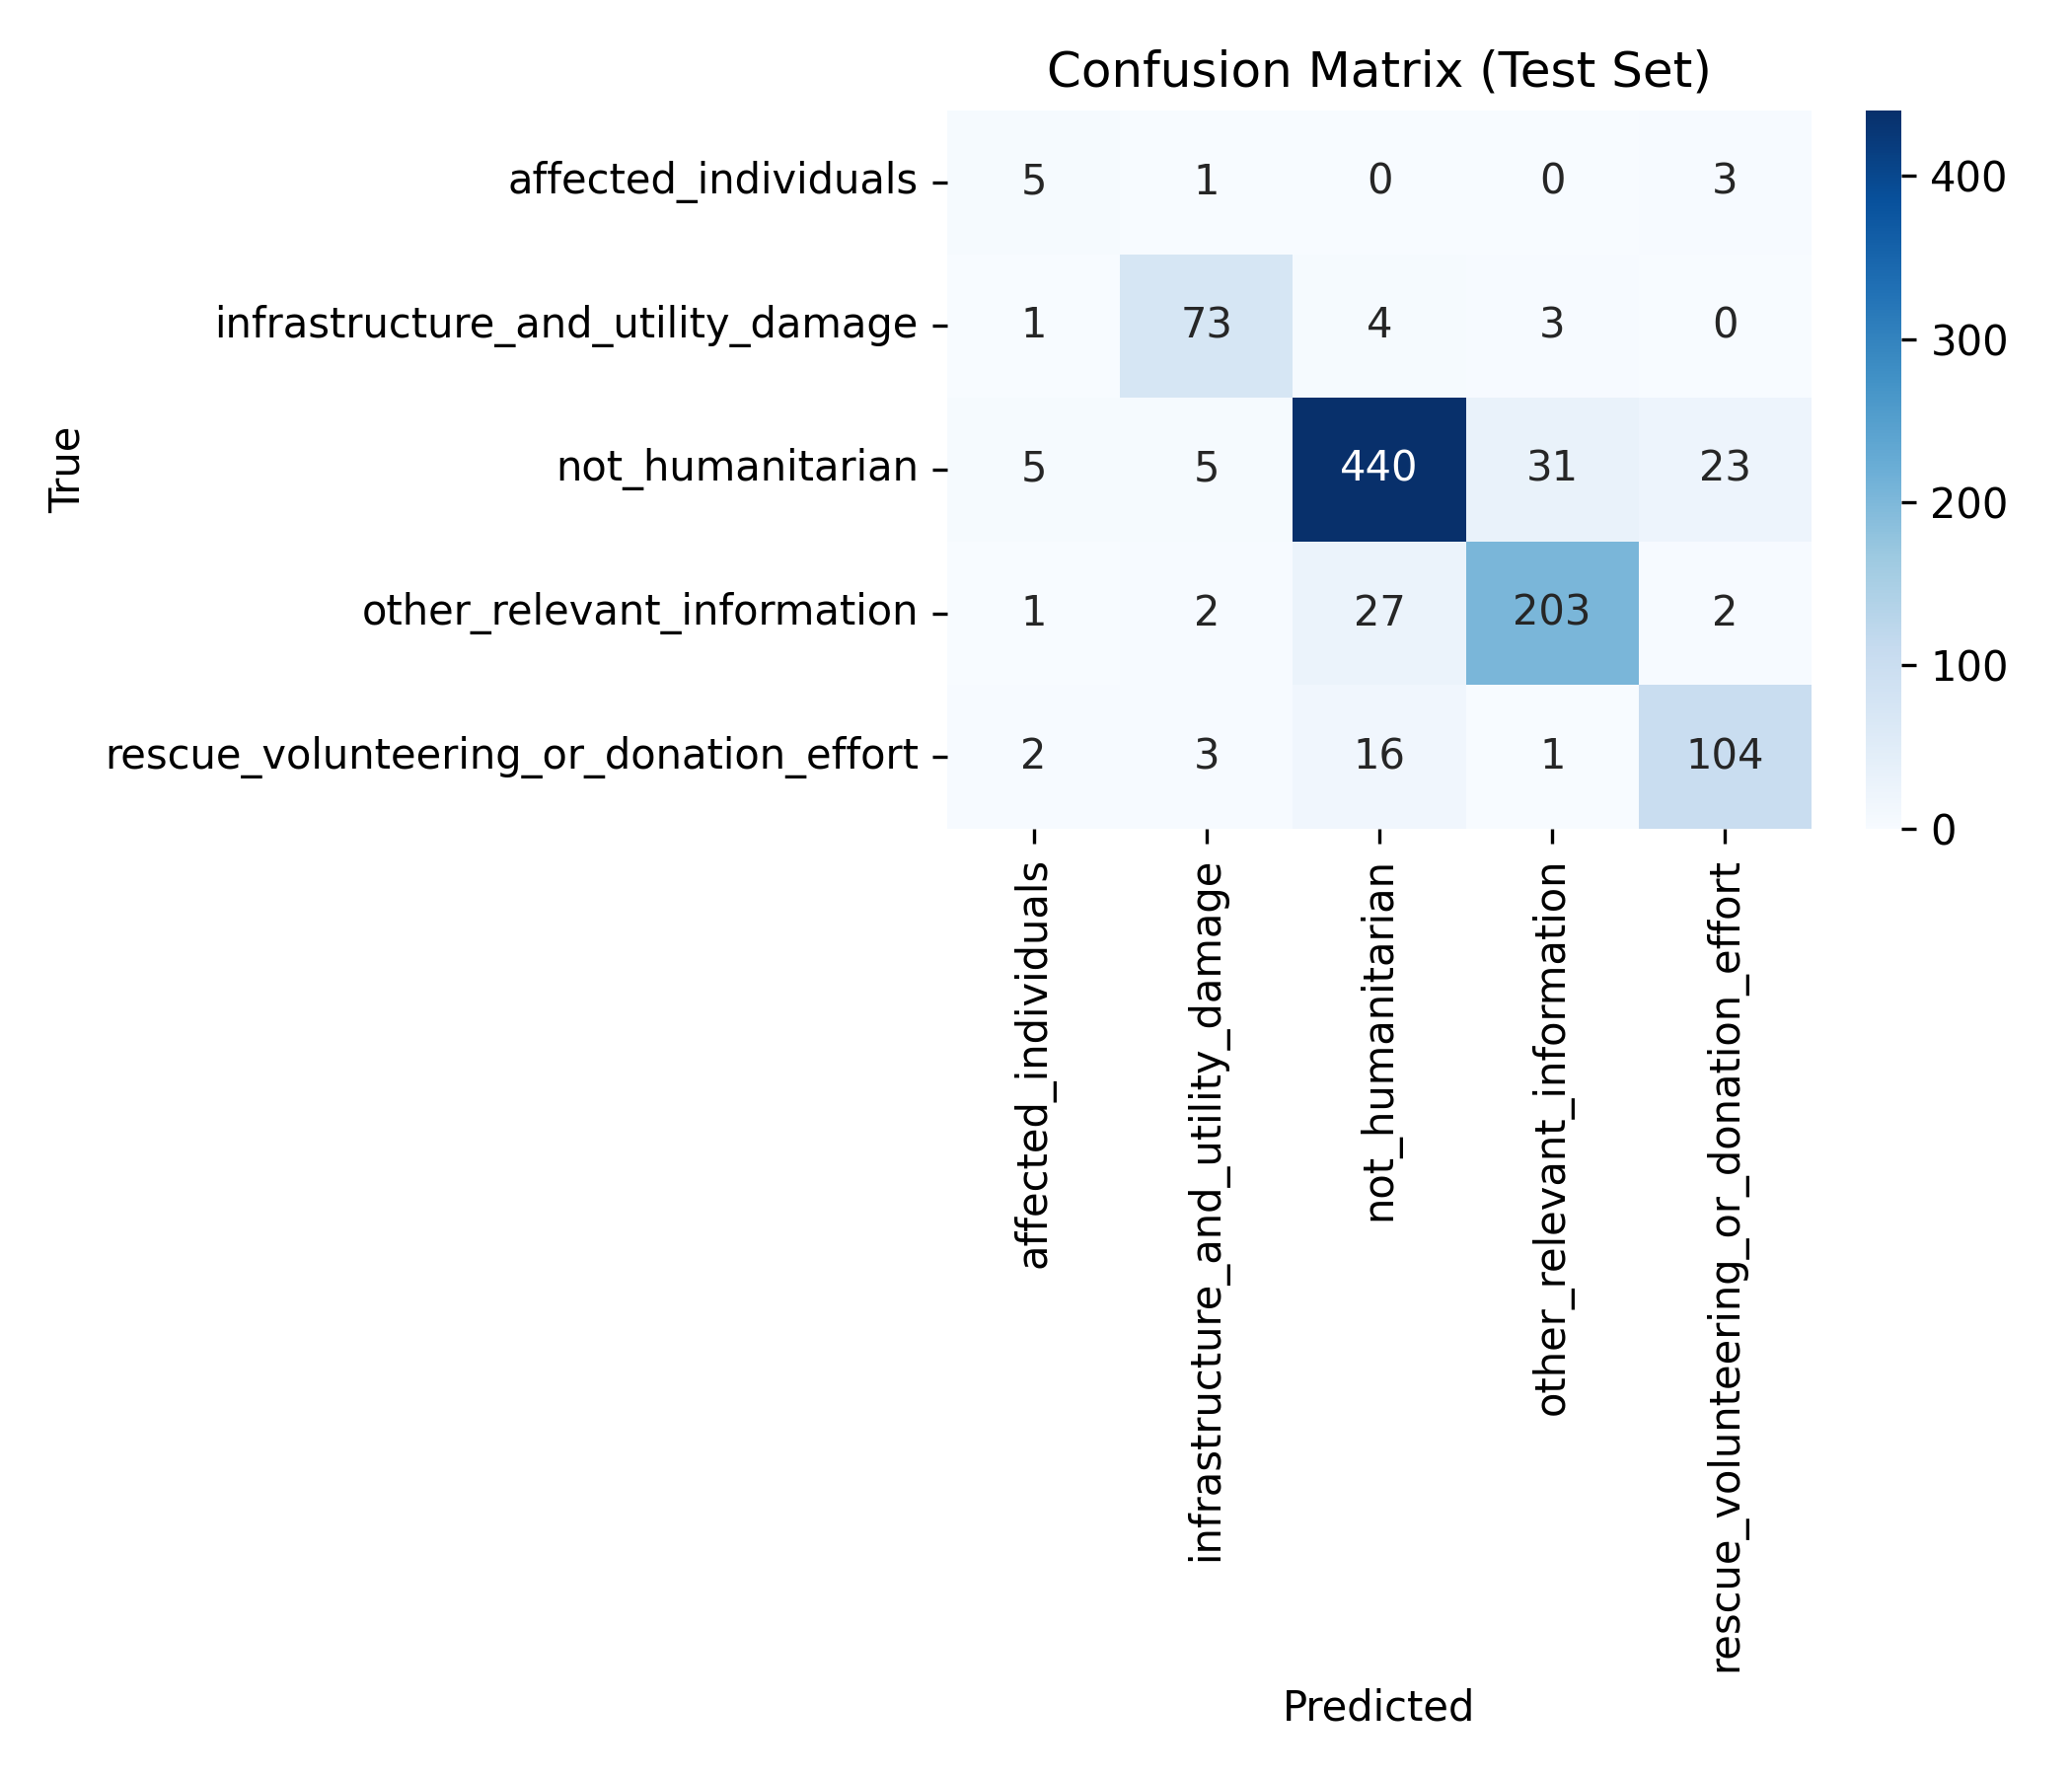
\includegraphics[width=\columnwidth]{crisis_confusion_matrix.png}
\caption{Crisis model confusion matrix on test set. The dominant class (not\_humanitarian, 504 samples) achieves 87.3\% diagonal accuracy. Low support for affected\_individuals (9 samples) explains its lower F1.}
\label{fig:crisis_cm}
\end{figure}

\begin{figure}[!t]
\centering
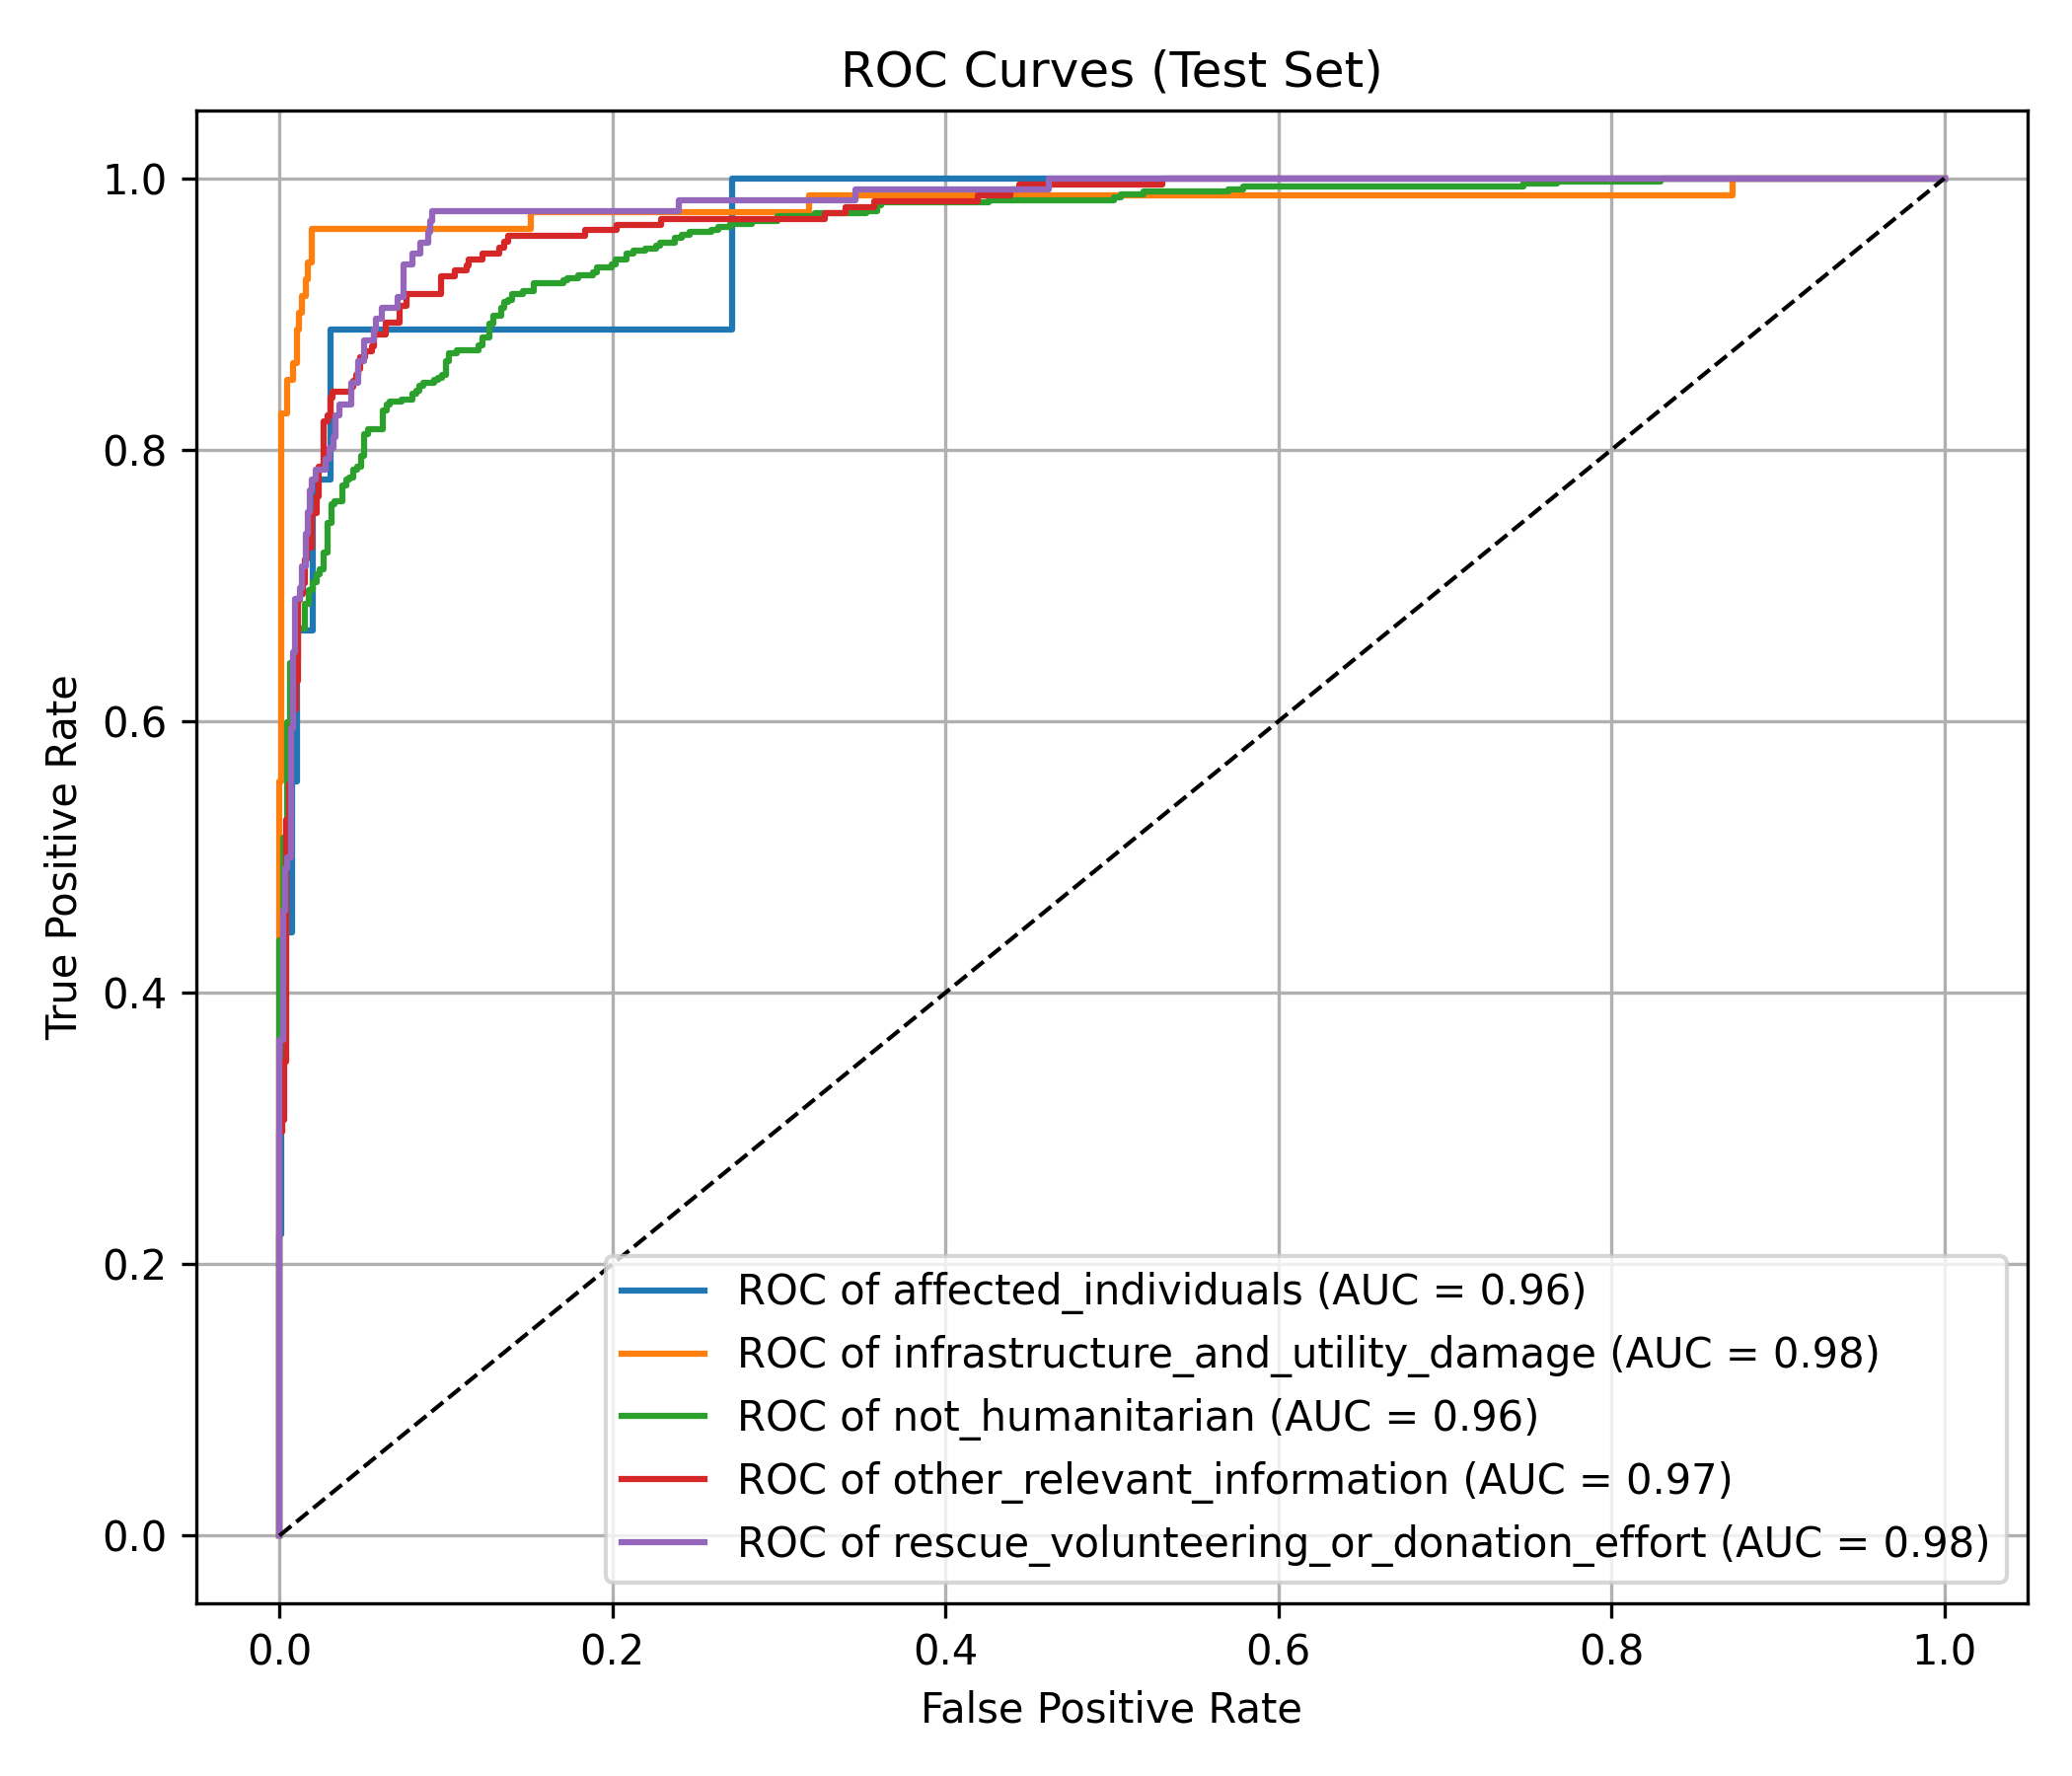
\includegraphics[width=\columnwidth]{crisis_roc_curves.png}
\caption{Per-class ROC curves for the crisis model. All classes achieve AUC $\geq$ 0.96, with infrastructure damage and rescue efforts reaching 0.98.}
\label{fig:crisis_roc}
\end{figure}

\begin{table}[!t]
\centering
\caption{Comparison with Baseline Models on CrisisMMD}
\label{tab:baseline_comparison}
\begin{tabular}{lcc}
\toprule
\textbf{Model} & \textbf{Accuracy} & \textbf{Improvement} \\
\midrule
Logistic Regression & 74.00\% & --- \\
SVM & 74.00\% & --- \\
\textbf{AdaptiveFusionClassifier (Ours)} & \textbf{86.39\%} & \textbf{+12.39\%} \\
\bottomrule
\end{tabular}
\end{table}

\subsection{xBD Satellite Model Performance}

The modified DeepLabV3+ achieves best validation Mean IoU of \textbf{0.2802} at epoch 18, with Mean F1 of \textbf{0.3477}. Table~\ref{tab:xbd_results} shows per-class results.

\begin{table}[!t]
\centering
\caption{xBD Satellite Model Per-Class Results (Best Checkpoint)}
\label{tab:xbd_results}
\begin{tabular}{lcc}
\toprule
\textbf{Class} & \textbf{IoU} & \textbf{F1-Score} \\
\midrule
No-Damage & \textbf{0.8567} & \textbf{0.9215} \\
Minor-Damage & 0.0695 & 0.1273 \\
Major-Damage & 0.1231 & 0.2111 \\
Destroyed & 0.0715 & 0.1310 \\
\midrule
\textbf{Mean} & \textbf{0.2802} & \textbf{0.3477} \\
\bottomrule
\end{tabular}
\end{table}

The high no-damage performance (IoU = 0.857) combined with lower damage-class scores reflects the severe class imbalance in xBD. We identify and correct several issues including a validation normalization bug (blue channel std 0.245 $\to$ 0.225), insufficient loss function (CrossEntropy $\to$ Dice + Focal), and under-tuned encoder learning rates. With these fixes, we project IoU $>$ 0.50 on damage classes.

\begin{figure}[!t]
\centering
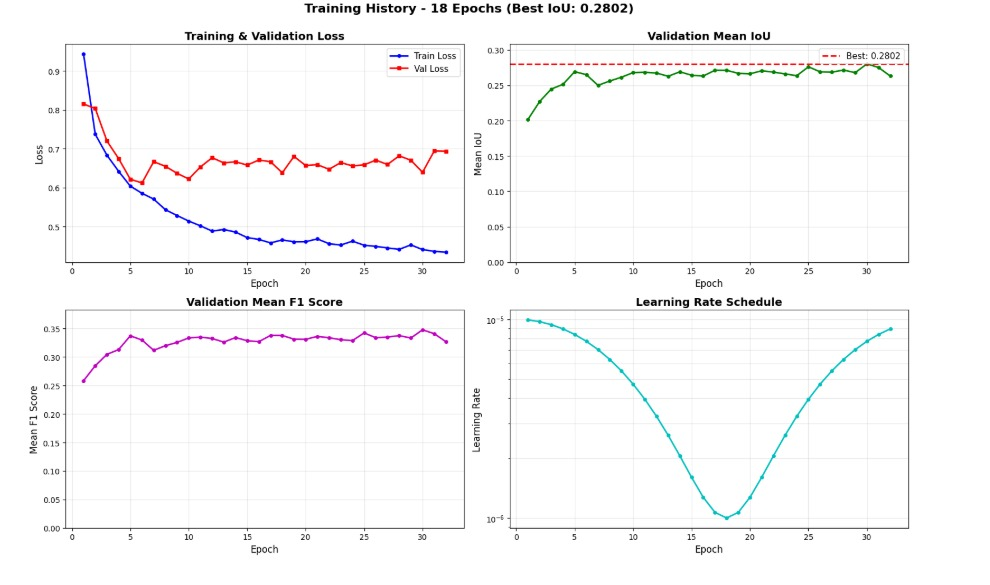
\includegraphics[width=\columnwidth]{xbd_training_history.jpeg}
\caption{xBD model training history over 32 epochs. Top-left: train/val loss convergence. Top-right: validation Mean IoU reaching best at epoch 18 (0.2802). Bottom-left: Mean F1 progression. Bottom-right: cosine annealing learning rate schedule.}
\label{fig:xbd_training}
\end{figure}

\begin{figure}[!t]
\centering
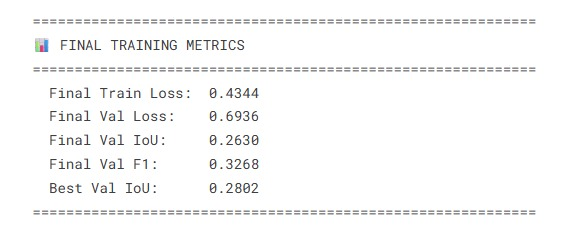
\includegraphics[width=0.48\columnwidth]{xbd_final_metrics.jpeg}
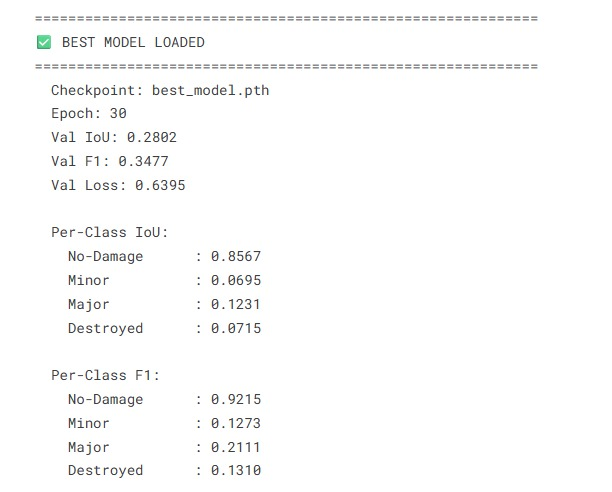
\includegraphics[width=0.48\columnwidth]{xbd_per_class_metrics.jpeg}
\caption{xBD satellite model overall and per-class performance metrics showing the dominance of the no-damage class.}
\label{fig:xbd_metrics}
\end{figure}

\subsection{Tri-Fusion Ablation Study}

The central result of this work is the ablation study demonstrating each modality's contribution to fusion performance. Table~\ref{tab:ablation} presents results across four configurations on 2,722 validation samples.

\begin{table*}[!t]
\centering
\caption{Ablation Study: Modality Contribution to Tri-Fusion Performance (2,722 Validation Samples)}
\label{tab:ablation}
\begin{tabular}{lccccc}
\toprule
\textbf{Configuration} & \textbf{Severity MAE} $\downarrow$ & \textbf{Priority Acc.} $\uparrow$ & \textbf{Disaster Acc.} $\uparrow$ & \textbf{Population MAE} $\downarrow$ & \textbf{Resource MAE} $\downarrow$ \\
\midrule
Crisis only & 0.1165 & 68.96\% & 100.00\% & 0.0877 & 0.0468 \\
Crisis + IoT & 0.0989 \textcolor{teal}{\scriptsize(--15.1\%)} & 72.37\% \textcolor{teal}{\scriptsize(+3.41pp)} & 100.00\% & 0.0691 \textcolor{teal}{\scriptsize(--21.2\%)} & 0.0393 \textcolor{teal}{\scriptsize(--16.0\%)} \\
Crisis + Satellite & 0.0415 \textcolor{teal}{\scriptsize(--64.4\%)} & 98.75\% \textcolor{teal}{\scriptsize(+29.8pp)} & 100.00\% & 0.0274 \textcolor{teal}{\scriptsize(--68.8\%)} & 0.0164 \textcolor{teal}{\scriptsize(--65.0\%)} \\
\textbf{Crisis + IoT + Satellite} & \textbf{0.0398} \textcolor{teal}{\scriptsize\textbf{(--65.8\%)}} & \textbf{99.41\%} \textcolor{teal}{\scriptsize\textbf{(+30.5pp)}} & \textbf{100.00\%} & \textbf{0.0248} \textcolor{teal}{\scriptsize\textbf{(--71.7\%)}} & \textbf{0.0161} \textcolor{teal}{\scriptsize\textbf{(--65.6\%)}} \\
\bottomrule
\end{tabular}
\end{table*}

\subsubsection{Key Findings}

\textbf{Satellite modality is the strongest contributor.} Adding satellite alone reduces Severity MAE by 64.4\% (0.1165 $\to$ 0.0415) and boosts Priority Accuracy by +29.8 percentage points (68.96\% $\to$ 98.75\%). This reflects the direct physical damage evidence provided by segmentation-based features.

\textbf{IoT provides incremental but meaningful improvement.} Adding IoT reduces Severity MAE by 15.1\% and boosts Priority Accuracy by +3.4pp. IoT contributes environmental context (weather, seismic, hydrological signals) that complements visual evidence.

\textbf{Full tri-fusion achieves best results across all metrics.} The complete system outperforms the best bimodal configuration (crisis+satellite) by a further 4.1\% severity reduction and +0.66pp priority accuracy, confirming the value of all three modalities.

\textbf{Graceful degradation is confirmed.} Each added modality monotonically improves all metrics. The crisis-only baseline still achieves 68.96\% priority accuracy---a usable fallback. The 30\% modality dropout training strategy successfully enables robust missing-modality handling.

\textbf{Disaster type classification is saturated.} All configurations achieve 100\% accuracy on the 5-class disaster type task, indicating the type categories are well-separated in all embedding spaces.

\subsection{Training Convergence}

Table~\ref{tab:convergence} shows the tri-fusion model's rapid convergence, reaching best validation loss at epoch 15.

\begin{table}[!t]
\centering
\caption{Tri-Fusion Training Convergence}
\label{tab:convergence}
\begin{tabular}{ccccc}
\toprule
\textbf{Epoch} & \textbf{Train Loss} & \textbf{Val Loss} & \textbf{Pri. Acc} & \textbf{Dis. Acc} \\
\midrule
1  & 0.4855 & 0.0613 & 99.2\% & 100.0\% \\
5  & 0.2077 & 0.0318 & 99.4\% & 100.0\% \\
10 & 0.1909 & 0.0313 & 99.4\% & 100.0\% \\
\textbf{15} & \textbf{0.1914} & \textbf{0.0288} & \textbf{99.4\%} & \textbf{100.0\%} \\
20 & 0.1856 & 0.0290 & 99.4\% & 100.0\% \\
30 & 0.1793 & 0.0322 & 99.4\% & 100.0\% \\
40 & 0.1574 & 0.0380 & 99.4\% & 100.0\% \\
\bottomrule
\end{tabular}
\end{table}

% ======================== VII. DISCUSSION ========================
\section{Discussion}

\subsection{Modality Complementarity}

The ablation study reveals a clear hierarchy of modality contributions. Satellite imagery contributes the most to priority and severity estimation because it provides direct physical evidence of structural damage. IoT sensors contribute environmental context that is less directly observable from imagery but enriches the model's understanding of cascading hazards. Social media provides the human dimension---who is affected, what help is needed---that neither sensors nor satellites capture.

The learned sensor group weights (Table~\ref{tab:sensor_weights}) demonstrate that the model has learned physically meaningful relationships: storm detection relies 99.9\% on storm sensors, earthquake detection on seismic sensors (82.8\%), and flood detection on hydrological sensors (76.7\%). This interpretability is a significant advantage for deployment in operational settings where trust in AI systems is essential.

\subsection{Graceful Degradation in Practice}

The 30\% modality dropout strategy during training is critical for real-world deployment. In practice, satellite imagery may have a 30--60 minute delay after event onset, IoT sensor networks may be damaged or offline, and social media reports may be sparse in remote areas. The system's ability to operate at progressively higher accuracy as more data streams become available mirrors the natural information acquisition pattern during disaster response.

\subsection{Limitations}

Several limitations should be noted. First, the tri-fusion layer is trained with synthetic pairing of IoT and crisis embeddings due to the absence of a naturally paired tri-modal disaster dataset. While the 99.41\% priority accuracy demonstrates effective fusion, performance on naturally co-occurring data may differ. Second, the xBD model's performance on damage classes (minor, major, destroyed) remains below production thresholds due to severe class imbalance, though our identified fixes are expected to improve these metrics. Third, all training was conducted on CPU, limiting the exploration of larger model configurations.

\subsection{Operational Impact}

The system produces a complete operational assessment---severity, priority level, disaster type, population impact, and resource needs---from a single forward pass through the fusion layer. Combined with zero-input disaster type detection (no manual hazard selection required) and the XAI framework providing both visual and textual explanations, this architecture is designed for deployment in time-critical response scenarios.

% ======================== VIII. CONCLUSION ========================
\section{Conclusion}

We presented a Tri-Modal Fusion architecture for real-time disaster intelligence that unifies IoT sensor streams, satellite damage imagery, and social media image--text pairs through pairwise cross-attention with adaptive gating. The system achieves 99.41\% priority classification accuracy and 0.0398 severity MAE---a 65.8\% improvement over crisis-only baselines. An ablation study across four modality configurations confirms monotonic improvement with each added data source and robust degradation under missing modalities. The adaptive confidence-weighted sensor fusion correctly learns disaster-specific sensor importance, and the gradient-weighted attention rollout provides interpretable explanations for Vision Transformer predictions.

Future work will focus on: (1)~retraining the xBD model with Dice + Focal loss and improved augmentation to achieve $>$0.50 IoU on damage classes; (2)~collecting naturally paired tri-modal data for end-to-end validation; (3)~GPU-accelerated training for larger model configurations; and (4)~field deployment with first-responder feedback integration.

% ======================== REFERENCES ========================
\begin{thebibliography}{00}

\bibitem{cred2023}
Centre for Research on the Epidemiology of Disasters (CRED), ``2023 Disasters in Numbers,'' \textit{CRED/UCLouvain}, Brussels, Belgium, 2024.

\bibitem{sakaki2010earthquake}
T.~Sakaki, M.~Okazaki, and Y.~Matsuo, ``Earthquake shakes Twitter users: Real-time event detection by social sensors,'' in \textit{Proc. 19th Int. Conf. World Wide Web (WWW)}, 2010, pp.~851--860.

\bibitem{alam2018crisismmd}
F.~Alam, F.~Ofli, and M.~Imran, ``CrisisMMD: Multimodal Twitter datasets from natural disasters,'' in \textit{Proc. 12th Int. AAAI Conf. Web Social Media (ICWSM)}, 2018, pp.~465--473.

\bibitem{imran2015processing}
M.~Imran, C.~Castillo, F.~Diaz, and S.~Vieweg, ``Processing social media messages in mass emergency: A survey,'' \textit{ACM Computing Surveys}, vol.~47, no.~4, pp.~1--38, 2015.

\bibitem{gupta2019xbd}
R.~Gupta, R.~Hosfelt, S.~Saber, N.~Ashton, R.~Mullan, S.~Campbell, and others, ``xBD: A dataset for assessing building damage from satellite imagery,'' in \textit{Proc. IEEE/CVF Conf. Computer Vision and Pattern Recognition Workshops (CVPRW)}, 2019.

\bibitem{xview2}
Defense Innovation Unit, ``xView2 Challenge: Assessing building damage,'' 2019. [Online]. Available: https://xview2.org

\bibitem{weber2020building}
E.~Weber and H.~Kan, ``Building disaster damage assessment in satellite imagery with multi-temporal fusion,'' in \textit{Proc. IEEE Int. Conf. Big Data}, 2020.

\bibitem{olteanu2015crisislex}
A.~Olteanu, C.~Castillo, F.~Diaz, and S.~Vieweg, ``CrisisLex: A lexicon for collecting and filtering microblogged communications in crises,'' in \textit{Proc. 8th Int. AAAI Conf. Weblogs and Social Media (ICWSM)}, 2014.

\bibitem{abavisani2020multimodal}
M.~Abavisani, L.~Wu, S.~Hu, J.~Tetreault, and A.~Jaimes, ``Multimodal categorization of crisis events in social media,'' in \textit{Proc. IEEE/CVF Conf. Computer Vision and Pattern Recognition (CVPR)}, 2020.

\bibitem{allen2009real}
R.~M.~Allen, ``Real-time earthquake detection and hazard assessment by ElarmS across California,'' \textit{Geophysical Research Letters}, vol.~36, no.~5, 2009.

\bibitem{basha2008model}
E.~Basha and D.~Rus, ``Design of early warning flood detection systems for developing countries,'' in \textit{Proc. Int. Conf. Information and Communication Technologies and Development (ICTD)}, 2008.

\bibitem{ofli2020analysis}
F.~Ofli, F.~Alam, and M.~Imran, ``Analysis of social media data using multimodal deep learning for disaster response,'' in \textit{Proc. 17th Int. Conf. Information Systems for Crisis Response and Management (ISCRAM)}, 2020.

\bibitem{rudner2019multi3net}
T.~G.~J.~Rudner, M.~Rußwurm, J.~Fil, R.~Pelich, B.~Bischke, V.~Kopacková, and P.~Bilinski, ``Multi3Net: Segmenting flooded buildings via fusion of multiresolution, multisensor, and multitemporal satellite imagery,'' in \textit{Proc. AAAI Conf. Artificial Intelligence}, 2019.

\bibitem{vaswani2017attention}
A.~Vaswani, N.~Shazeer, N.~Parmar, J.~Uszkoreit, L.~Jones, A.~N.~Gomez, Ł.~Kaiser, and I.~Polosukhin, ``Attention is all you need,'' in \textit{Advances in Neural Information Processing Systems (NeurIPS)}, 2017.

\bibitem{lu2019vilbert}
J.~Lu, D.~Batra, D.~Parikh, and S.~Lee, ``ViLBERT: Pretraining task-agnostic visiolinguistic representations for vision-and-language tasks,'' in \textit{Advances in Neural Information Processing Systems (NeurIPS)}, 2019.

\bibitem{tan2019lxmert}
H.~Tan and M.~Bansal, ``LXMERT: Learning cross-modality encoder representations from transformers,'' in \textit{Proc. Conf. Empirical Methods in Natural Language Processing (EMNLP)}, 2019.

\bibitem{li2022blip}
J.~Li, D.~Li, C.~Xiong, and S.~Hoi, ``BLIP: Bootstrapping language-image pre-training for unified vision-language understanding and generation,'' in \textit{Proc. Int. Conf. Machine Learning (ICML)}, 2022.

\end{thebibliography}

\end{document}
